% !TeX program = xelatex
\documentclass[a4paper,11pt,oneside]{article}

%%%%%%%%%%%%%%%%%%%%%
% Encodage et langues
\usepackage[numbers]{natbib}
\usepackage[main=french,english]{babel}
\usepackage{fontspec}
\usepackage{xeCJK}
\setCJKmainfont{FandolSong}
\setCJKsansfont{FandolHei}
\setCJKmonofont{FandolFang}

%%%%%%%%%%%%%%%%%%%%%
% Liens et métadonnées
\usepackage[colorlinks=false, breaklinks, pdfborder={0 0 0}]{hyperref}

%%%%%%%%%%%%%%%%%%%%%
% Mise en page et utilitaires
\usepackage{float}
\usepackage{amsmath}
\usepackage{amssymb}
\usepackage{geometry}
\geometry{a4paper, margin=2.5cm, headheight=17pt}
\usepackage{graphicx}
\usepackage{caption}
\usepackage{booktabs}
\usepackage{longtable}
\usepackage{listings}
\usepackage{array}
\usepackage{tikz}
\usetikzlibrary{positioning,calc}
\usepackage{pgfplots}
\pgfplotsset{compat=1.18}
\usepackage{xcolor}
\usepackage{enumitem}
\usepackage{fancyhdr}
\usepackage{setspace}
\usepackage{titlesec}

% Rendre les listes moins "visuelles" et plus compactes (réduit la fatigue à la lecture)
\setlist[itemize]{label=\textendash, leftmargin=*, nosep}

\lstset{
	    basicstyle=\ttfamily\footnotesize,
	    breaklines=true,
	    frame=single,
    backgroundcolor=\color{gray!5},
    literate={é}{{\'e}}1 {è}{{\`e}}1 {à}{{\`a}}1 {ç}{{\c{c}}}1 {œ}{{\oe}}1 {ù}{{\`u}}1 {É}{{\'E}}1 {È}{{\`E}}1 {À}{{\`A}}1 {Ç}{{\c{C}}}1 {Œ}{{\OE}}1 {Ê}{{\^E}}1 {ê}{{\^e}}1 {î}{{\^i}}1 {ô}{{\^o}}1 {û}{{\^u}}1
}

\lstdefinelanguage{pseudo}{
    morekeywords={for,foreach,while,if,else,return},
    sensitive=false
}

\newcommand{\bigO}[1]{\ensuremath{\mathop{}\mathopen{}O\mathopen{}\left(#1\right)}}
\newcommand{\smallO}[1]{\ensuremath{\mathop{}\mathopen{}o\mathopen{}\left(#1\right)}}

\captionsetup[figure]{font=footnotesize, justification=centering, singlelinecheck=true, position=bottom}
\captionsetup[table]{font=footnotesize, justification=centering, singlelinecheck=true, position=bottom}
\urlstyle{same}
\emergencystretch=1em

\setcounter{tocdepth}{3}
\setcounter{secnumdepth}{3}
\setstretch{1.0}
\setlength{\parindent}{2em}
\setlength{\parskip}{0pt}
\renewcommand{\contentsname}{目录}
\renewcommand{\bibname}{参考文献}

\titleformat{\section}
  {\normalfont\fontsize{18pt}{24pt}\selectfont\bfseries}
  {\thesection}
  {0.8em}
  {}
\titlespacing*{\section}{0pt}{1.8em}{0.8em}

\titleformat{\subsection}
  {\normalfont\fontsize{14pt}{19pt}\selectfont\bfseries}
  {\thesubsection}
  {0.7em}
  {}
\titlespacing*{\subsection}{0pt}{1.2em}{0.5em}

\titleformat{\subsubsection}
  {\normalfont\fontsize{12pt}{16pt}\selectfont\bfseries}
  {\thesubsubsection}
  {0.6em}
  {}
\titlespacing*{\subsubsection}{0pt}{0.9em}{0.35em}

\newcommand{\reporttype}{项目报告}
\newcommand{\reporttitletext}{应用于 MNIST 的 MLP 与自动微分引擎}
\newcommand{\reportshorttitle}{MLP 与自动微分引擎}
\newcommand{\reportinstitution}{Université de Versailles Saint-Quentin-en-Yvelines}
\newcommand{\reportprogram}{Master CHPS -- UVSQ}
\newcommand{\reportyear}{2025--2026}
\newcommand{\reportheadertext}{Master CHPS -- UVSQ 2025 - 2026}
\newcommand{\reportauthorsblock}{%
  \begin{tabular}{@{}>{\raggedright\arraybackslash}p{0.66\textwidth}@{}}
    \textbf{Jianye Shi} \\
    \href{mailto:jianye.shi@ens.uvsq.fr}{jianye.shi@ens.uvsq.fr} \\
    \\[-0.2em]
    \textbf{Hao Qian} \\
    \href{mailto:hao.qian@ens.uvsq.fr}{hao.qian@ens.uvsq.fr} \\
    \\[-0.2em]
    \textbf{Xiang Bian} \\
    \href{mailto:xiang.bian@ens.uvsq.fr}{xiang.bian@ens.uvsq.fr} \\
    \\[-0.2em]
    \textbf{Abdennour Boulmis} \\
    \href{mailto:abdennour.boulmis@ens.uvsq.fr}{abdennour.boulmis@ens.uvsq.fr}
  \end{tabular}%
}
\newcommand{\reportadvisor}{Aurélien Delval}
\newcommand{\reportdate}{2026 年 4 月 29 日}

%%%%%%%%%%%%%%%%%%%%%
% En-têtes et pieds de page
\fancyhf{}
\fancyhead[L]{\textit{\reportheadertext}}
\fancyhead[R]{\nouppercase{\rightmark}}
\fancyfoot[C]{\thepage}
\renewcommand{\headrulewidth}{0.4pt}
\renewcommand{\footrulewidth}{0pt}
\setlength{\headheight}{17pt}
\renewcommand{\sectionmark}[1]{\markright{\thesection.\ #1}}
\fancypagestyle{plain}{
  \fancyhf{}
  \fancyfoot[C]{\thepage}
  \renewcommand{\headrulewidth}{0pt}
  \renewcommand{\footrulewidth}{0pt}
}

\begin{document}

\hypersetup{pageanchor=false}
\pagenumbering{gobble}
\begin{titlepage}
  \thispagestyle{empty}
  \noindent
  \begin{minipage}[t]{0.60\textwidth}
    \vspace*{0pt}
    {\Large\bfseries \reportinstitution\par}
    \vspace{0.35cm}
    {\normalsize Faculté des sciences et ingénierie\par}
    \vspace{0.55cm}
    {\color{black!55}\rule{0.76\textwidth}{0.8pt}\par}
  \end{minipage}
  \hfill
  \begin{minipage}[t]{0.22\textwidth}
    \vspace*{-0.2cm}
    \raggedleft
    
\includegraphics[width=\textwidth]{Images/Logo_UVSQ.jpg}
  \end{minipage}

  \vspace{2.4cm}

  {\fontsize{22pt}{28pt}\selectfont\bfseries \reporttitletext\par}
  \vspace{0.45cm}
  {\Large\color{black!70} \reporttype\par}

  \vspace{1.6cm}

  \begin{minipage}[t]{0.58\textwidth}
    \raggedright
    {\small\scshape Auteurs\par}
    \vspace{0.45cm}
    {\normalsize \reportauthorsblock\par}
  \end{minipage}
  \hfill
  \begin{minipage}[t]{0.32\textwidth}
    \raggedright
    {\small\scshape Encadrement\par}
    \vspace{0.45cm}
    {\normalsize\textbf{Aurélien Delval}\par}
    \vspace{0.25cm}
    {\small Enseignant-chercheur\par}
  \end{minipage}

  \vfill
  \noindent{\color{black!55}\rule{\textwidth}{0.8pt}\par}
  \vspace{0.35cm}
  \noindent
  \begin{minipage}[t]{0.48\textwidth}
    \raggedright
    {\small \reportprogram}
  \end{minipage}
  \hfill
  \begin{minipage}[t]{0.32\textwidth}
    \raggedleft
    {\small \reportdate}
  \end{minipage}
\end{titlepage}

\clearpage
\hypersetup{pageanchor=true}
\pagenumbering{roman}
\setcounter{page}{1}
\tableofcontents
\clearpage
\pagenumbering{arabic}
\setcounter{page}{1}
\pagestyle{fancy}

\section{引言}

\subsection{项目背景与研究对象}
神经网络系统的实现不仅涉及模型结构本身，也涉及训练运行时、数值计算内核以及数据输入路径等多个层面。以图像分类任务为载体，从零实现一套可训练的神经网络程序，有助于在统一代码基础上考察前向传播、反向传播、参数更新与实验执行流程之间的关系，并为后续的性能测量与实现比较提供可控环境。

本报告讨论的对象是一个以 C++ 为基础实现的神经网络实验系统。该系统当前覆盖了多层感知机（MLP, multi-layer perceptron）与卷积神经网络（CNN, convolutional neural network）两类模型路径，同时包含自动微分运行时、矩阵乘法与卷积计算后端、数据加载接口，以及面向分布式训练实验的同步机制。本文关注的是这些组成部分在当前实现范围内的组织方式、扩展方向与实验用途，而非将其表述为通用深度学习框架或稳定完备的训练平台。

\subsection{前期基础与本阶段扩展}
前期工作已经完成了基于 MNIST \cite{lecun1998} 的多层感知机训练基础，包括反向模式自动微分、显式计算图、基础矩阵计算核心与完整训练循环。该部分工作提供了可运行的功能基线，也为后续比较不同计算实现、扩展卷积路径以及观察运行时开销提供了统一的实验起点。

在此前基础上，本阶段将系统从单一的 MLP/MNIST 原型扩展为能够承载更多技术路径的实验对象。扩展内容主要包括：加入可配置的 CNN 路径，以支持卷积模型实验；围绕通用矩阵乘法（GEMM, general matrix multiplication）与卷积相关算子进行实现比较与优化；整理自动微分运行时，以便更清晰地区分框架层开销与算子层开销；引入 Tiny-ImageNet 数据集路径，用于评估当前实现对更高负载图像输入与训练流程的适配范围；并加入基于消息传递接口（MPI, message passing interface）的同步数据并行实验路径，用于考察分布式梯度同步在当前实现中的组织方式与边界。

\subsection{报告范围与后文内容}
本文后续内容围绕上述扩展依次展开。首先讨论 GEMM 相关实现及其比较方法，并据此说明后续实验中复用的矩阵计算配置；随后介绍卷积路径与 CNN 结构在当前代码中的实现范围；在此基础上，再说明 Tiny-ImageNet 数据集接入、输入管线与训练支撑代码的组织方式；最后讨论 MPI 分布式同步路径和自动微分运行时整理的相关内容。附录部分补充若干诊断实验与参数推导过程，用于支持正文中的实现分析与实验解释。

\section{GEMM矩阵乘法算子的优化}

在当前系统中，GEMM（general matrix multiplication，通用矩阵乘法）是核心底层计算算子，同时用于 MLP 的全连接层和卷积路径中的 \texttt{im2col + matmul} 方案。因此，其实现效率会直接影响 CNN、Tiny-ImageNet 和分布式训练实验的总体耗时。

本章围绕项目中的多种 GEMM 路径展开实现、比较与优化，包括 \texttt{blas}（OpenBLAS）、\texttt{omp}（上学期实现的基础 OpenMP 版本）、\texttt{omp\_blocked}、\texttt{omp\_blocked\_packab}、\texttt{omp\_gotoblas\_avx2} 和 \texttt{omp\_gotoblas\_avx512}。目标是结合 OpenMP 并行、cache blocking（缓存分块）、packing（数据打包）和 GotoBLAS 风格分层加 SIMD 微内核，使 GEMM workload 更适配当前设备。

具体而言，本章关注的问题包括：基础 OpenMP 并行能带来多少收益，cache blocking（缓存分块）与 packing（数据打包）是否能够改善访存行为，GotoBLAS 风格的分层结构在本项目的 workload（工作负载）上是否有效，以及 AVX2/AVX-512 微内核在不同矩阵形状和线程数下表现是否稳定。相关结果主要用于形成后续实验中复用的 \texttt{matmul} 实现配置。

\subsection{实验环境}
除特别说明外，本章后续实验均使用附录~\ref{app:gemm_setup} 中列出的硬件环境、软件配置、测量协议和 CPU 绑定设置。GEMM 比较默认采用 1 至 8 线程配置，对应 8 个物理核心，并启用 \texttt{OMP\_PROC\_BIND=true} 与 \texttt{OMP\_PLACES=cores}；只有 SMT/超线程对照实验使用 16 线程配置。

\subsection{线程预算与实验协议}\label{sec:gemm_smt}

在正式比较各 GEMM 实现之前，先通过一组 SMT 对照实验确定线程预算。对照实验的结论是：16 线程（SMT）配置在 OpenBLAS 和基础 OpenMP 实现上均出现性能退化，主要原因是调度与同步等待开销在超线程共享的物理执行单元上被放大（详见附录~\ref{app:smt_diagnosis}）。

\textbf{因此，后续所有实验均沿用这一基准配置，}以避免 SMT 配置下的调度波动混入 backend 比较。施加亲和性约束后的线程扩展性对比见附录~\ref{app:smt_diagnosis}。

\subsection{OpenMP分块与打包技术}

相对于 \texttt{omp} 基线，本节关注 \textbf{分块（Blocking）}与\textbf{数据打包（Packing）}在并行执行时能在多大程度上进一步改善各线程的工作局部性。

从时间局部性（temporal locality）的角度看，blocking 的目的，是在子块被逐出前尽可能复用已进入 cache 的 $A$、$B$ 与 $C$ 子块。否则，尚未充分利用的数据就会被后续访问的新数据替换。

packing 则是在 blocking 之外，将后续需要反复读取的面板（panel）或子块复制到连续缓冲区中并重新排列。这样可以用一次额外复制换取更规则的顺序访存、更少的 stride 访问和更可控的 cache residency（缓存驻留），从而减少 cache / TLB miss 并提高带宽利用率。

具体调参与筛选过程见附录~\ref{app:blocked_pack_screening}；在当前平台上，\texttt{omp\_blocked} 更接近 L2-oriented blocking，而带 packing 的路径则更接近 L1-oriented 设计。

基于这一点，下面转向结构更完整的 GotoBLAS 风格路径，并继续考察其在当前设备与工作负载上的适配效果。

\subsection{GotoBLAS架构}\label{sec:gotoblas_arch}

前述 packing 优化已经改善了数据局部性，也为寄存器级计算提供了基础。在此之上，后续实现进一步引入微内核，以在 GotoBLAS 风格组织下更有效地利用寄存器层面的 SIMD。

\subsubsection{三层分块模型}

GotoBLAS 将 $C = A \cdot B$（规模 $M \times K \times N$）分解为三层嵌套循环及最内层微内核，如图~\ref{fig:gotoblas_overview} 所示。

\begin{figure}[H]
    \centering
    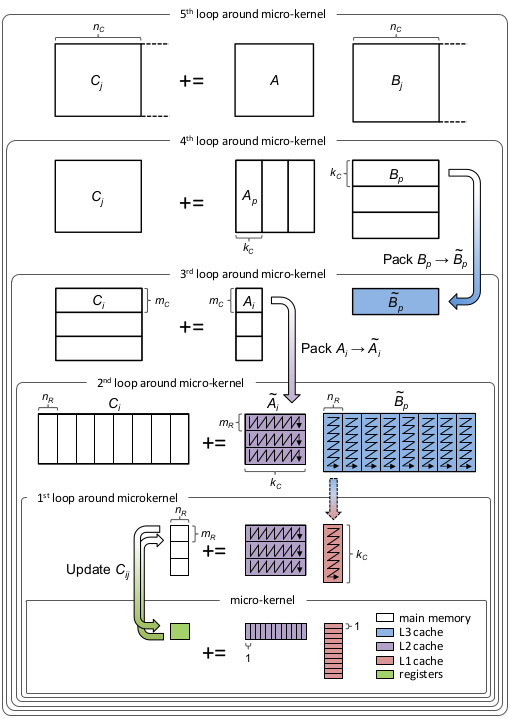
\includegraphics[width=0.48\textwidth]{Images/blis_design.png}
    \hfill
    
\includegraphics[width=0.48\textwidth]{Images/DataMovement.png}
    \caption{左：围绕微内核组织的 GotoBLAS/BLIS 风格 GEMM 分层结构，转引自 \cite[Fig.~1]{vanzee2017complex}。右：BLIS/GotoBLAS 实现中数据移动与面板在内存层次中放置方式的示意图，转引自 \cite[Fig.~4]{low2016analytical}。}
    \label{fig:gotoblas_overview}
\end{figure}

外层三层 blocking 与 packing 的作用，是将工作集压缩并稳定驻留在合适的 cache 层级中；最内层 micro-kernel 则在寄存器层面最大化对这些 packed 数据的复用。

\begin{enumerate}
    \item \textbf{外层（$N_c$维度）}：沿 $N$ 维以 $N_c$ 为步长，将 $B$ 的面板（$K \times N_c$）装入 LLC（L3 缓存）；
    \item \textbf{中层（$K_c$维度）}：沿 $K$ 维以 $K_c$ 为步长，将打包后的 $B$ 面板（$K_c \times N_c$）装入 L2 缓存；
    \item \textbf{内层（$M_c$维度）}：沿 $M$ 维以 $M_c$ 为步长，将打包后的 $A$ 面板（$M_c \times K_c$）装入 L1 缓存；
    \item \textbf{微内核（$M_r \times N_r$寄存器 tile）}：最内层操作，在 SIMD 寄存器中累积 $M_r \times N_r$ 的 $C$ 块。
\end{enumerate}

需要说明的是，这一层次化模型默认各层块都能形成足够规整的 tile；但当 $M$ 很小或线程数较高时，沿 $M$ 维切分后每个线程实际分得的行数可能低于微内核高度 $M_r$。此时宏块与寄存器块无法充分铺满，程序会更频繁地落入边界处理（remainder loop），从而削弱三层分块本应带来的缓存复用与并行效率。

缓存块参数按面板容量估算：$A$ 面板 $M_c \times K_c \times 4$ 字节对应 L1（32~KiB/核），$B$ 面板 $K_c \times N_c \times 4$ 字节对应 L2（1~MiB/核）。当前默认参数为 $K_c=384$、$M_c$ 有效行数 $=64$（倍率 8，基于 $M_r=8$）、$N_c=448$；这些参数在第~\ref{sec:avx2_tuning}节中继续做实验筛选。

\subsection{GotoBLAS调优与多线程并行策略}\label{sec:avx2_tuning}

参数搜索以项目中的神经网络 GEMM 形状为对象。由于 $(M_r,N_r,K_c,M_c,N_c)$ 的组合空间过大，本文采用分阶段筛选：先缩减候选，再对保留形状做单线程实验。

\subsubsection{微内核设计}\label{subsec:microkernel}

当前 AVX2 单精度微内核沿 $N$ 方向按 8 列组织，以匹配 YMM 向量宽度并减少边界处理。对 \texttt{float32} 路径而言，256 位 YMM 寄存器一次可覆盖 8 个 \texttt{float}，因此本实现优先筛选 $N_r$ 为 8 倍数的形状。

参数搜索协议、$(M_r,N_r,K_c,M_c,N_c)$ 搜索空间的缩减过程，以及分 workload 的详细结果统一放入附录~\ref{app:gemm_setup}、\ref{app:avx2_tuning_results} 和~\ref{app:blocked_size_tuning}。正文这里只保留后续多线程实验需要用到的结论。

\subsubsection{结果摘要}

在单线程下，\texttt{4x16} 与 \texttt{8x8} 是最有竞争力的两种微内核形状。前者在多种全连接层形状上更强，后者则在部分卷积相关 workload 上更稳。代表性的单线程形状对比图与各工作负载族的最佳配置汇总见附录中的图~\ref{fig:avx2_kernelshape_line} 与表~\ref{tab:avx2_tuning_results}。

相对于 OpenBLAS，主流形状（$N \geq 64$）的差距通常在 10 至 24\% 之间；而在极小 $N$ 的形状上，这一差距会扩大到 66 至 78\%，因为边界处理会占据更大比例。为了在后续多线程实验中使用一组固定配置，AVX2 路径最终采用 \texttt{avx2\_8x8} 作为主要折中方案。

\subsubsection{最终AVX2配置与AVX-512简介}\label{sec:avx512_brief}

基于上述单线程折中结果，后续多线程实验固定使用如下 AVX2 配置：
\[
\texttt{avx2\_8x8},\quad K_c = 384,\quad M_c = 64,\quad N_c = 448
\]
其中$M_c=64$为有效行数（代码常量 \texttt{kCacheBlockM}$=8$，有效值$= \texttt{kCacheBlockM} \times M_r = 8 \times 8 = 64$）。
该配置作为多线程比较中的固定基线。

AVX-512 路径沿用同一 \texttt{float32}/\texttt{Scalar=float} 数据路径，并采用 \texttt{avx512\_8x32} 微内核。最终选定：$\texttt{avx512\_8x32},\ K_c=160,\ M_c=64,\ N_c=448$（$M_c$ 有效行数为 64；$K_c=160$ 为实验调优值，通过 \texttt{MATMUL\_KC=160} 在运行时传入，与 AVX2 路径的编译常量 \texttt{kCacheBlockK}$=384$ 性质不同）。
AVX2 blocked-size 候选集合的详细推导见附录~\ref{app:blocked_size_tuning}。

\subsubsection{GotoBLAS多线程并行策略与参数调优}\label{sec:gotoblas_mt}

单线程调优确定了最优内核形状和块参数。进入多线程场景后，当前实现继续使用运行时给定的 $M_c, N_c, K_c$ 作为缓存分块参数，并在并行调度层引入随线程数变化的任务粒度：代码在 $ic/M$ 维上根据线程数计算更细的 \texttt{task\_m}，以便在小规模矩阵下产生更多任务，减少线程空闲。

\subsubsection{线程感知块参数调优}

在当前代码中，线程感知主要体现在调度粒度而非缓存块参数本身。也就是说，进入并行区后程序会根据线程数计算更细的 \texttt{task\_m}，而强扩展性实验本身只使用最终选定的固定 blocked-size 配置，不再展开其中间调参与推理过程。

本文后续强扩展性实验采用的固定配置为：AVX2 路径使用 $\texttt{avx2\_8x8},\ K_c=384,\ M_c=64,\ N_c=448$，AVX-512 路径使用 $\texttt{avx512\_8x32},\ K_c=160,\ M_c=64,\ N_c=448$。其中 $M_c=64$ 为有效行数（代码常量 \texttt{kCacheBlockM}$=8$，有效值$= 8 \times M_r = 8 \times 8 = 64$）。代表性的线程感知 \texttt{kCacheBlockM}/$N_c$ 热图见附录图~\ref{fig:mc_nc_heatmap_t4}；从该图可见，高性能区域集中在 \texttt{kCacheBlockM}$=8$（即有效 $M_c=64$）一行，而 $N_c$ 方向表现为相对平坦的平台。

\subsubsection{强扩展性实验（Strong Scaling）}

以固定问题规模、变化线程数（$T \in \{1,2,4,8\}$）的强扩展性实验，
对比了AVX2 GotoBLAS、AVX-512 GotoBLAS与OpenBLAS三种实现，
测试集涵盖9个工作负载（MLP、CNN卷积和方阵形状）。

\begin{figure}[H]
    \centering
    \includegraphics[width=0.82\textwidth]{../output/ExperienceGEMM/GotoBLASBlockedAVX512/fixed_strong_scaling_comparison/summary/plots/overall_geomean_gflops_by_threads.png}
    \caption{强扩展性实验：各线程数下的几何平均GFLOPS（跨9个工作负载）。}
    \label{fig:strong_scaling_geomean}
\end{figure}

图~\ref{fig:strong_scaling_geomean} 的统计口径是 9 个 fixed-config workload 的几何平均。按这一口径，8 线程下 AVX2 和 AVX512 GotoBLAS 的 speedup 均约为 $3.23\times$，而 OpenBLAS 约为 $2.72\times$。逐 workload 的结果则来自 fixed-config strong-scaling comparison：在多数 workload 上，OpenBLAS 的绝对 GFLOPS 更高；GotoBLAS 路径主要用于比较 blocking、packing 和 OpenMP 组织，并在部分方阵和少数卷积相关 GEMM 形状上保持竞争力。

\subsection{Unrolled+Prefetch实现思路}

在 AVX-512 路径完成基础调优后，代码又增加了一条 \textbf{unrolled+prefetch} 变体。该路径保留原有 blocked+packed 结构，只在 AVX-512 微内核及其对应的 packed panel 访问阶段加入循环展开（如 \texttt{GEMM\_UNROLL\_4}）和显式预取，从而进一步压缩最内层执行阶段的访存等待。它作用于 packed $A/B$ 面板的连续访问路径，统计范围仍与前文相同。

固定方阵上的补充线程扩展实验主要用于观察合成尺寸上的行为，因此放入附录~\ref{app:fixed_square_scaling}。


\section{损失函数、优化器与训练循环}

在当前主训练入口中，损失函数固定为 \texttt{CrossEntropyLoss}：模型前向输出类别 logits，损失层在内部执行数值稳定的 softmax 与交叉熵计算，并返回整个 batch 的标量 loss。代码中也保留了 \texttt{MSELoss} 实现，但当前分类路径统一使用 \texttt{CrossEntropyLoss}。

优化器方面，当前实现了 \texttt{SGD}、\texttt{MomentumSGD} 和 \texttt{AdamW} 三条路径。图~\ref{fig:optimizer_compare} 汇总了三种优化器在 MNIST MLP 上的 20 epoch 训练曲线。

\begin{figure}[h]
\centering
\includegraphics[width=0.92\textwidth]{../output/compare_opt/optimizer_compare.png}
\caption{三种优化器在 MNIST MLP（20 epoch）上的训练/测试损失与准确率对比。SGD 最终测试准确率 96.52\%，MomentumSGD 98.27\%，AdamW 98.03\%。}
\label{fig:optimizer_compare}
\end{figure}

三者的实现思路分别对应不同的参数更新机制。对于 \texttt{SGD}，参数按当前梯度直接更新：
\[
\theta_{t+1}=\theta_t-\eta g_t.
\]
\texttt{MomentumSGD} 在此基础上引入速度项，用指数平滑的历史梯度稳定更新方向：
\[
v_{t+1}=\mu v_t-\eta g_t,\qquad \theta_{t+1}=\theta_t+v_{t+1},
\]
并可按配置启用 Nesterov 修正。\texttt{AdamW} 则进一步维护梯度的一阶矩与二阶矩估计，并把 weight decay 从自适应更新中解耦，从而在保持收敛稳定性的同时改善正则化行为。

训练配置在构图完成后根据命令行参数选择优化器，并在每个训练 step 中先清空梯度，再在 backward 与可能的分布式同步完成后，按全局 batch 大小做缩放并执行参数更新。\texttt{Trainer::runEpoch(...)} 统一承担训练与评估两条路径：前者执行前向、损失计算、反向传播与参数更新，后者只保留前向与指标统计。因此，损失函数、优化器与训练循环构成了后续 CNN、ResNet 与分布式实验共享的同一训练主线。

\section{卷积算子的实现和优化}

本节为未来 CNN 中的卷积进行实现，重点分析 \texttt{im2col/GEMM/col2im} 主链路的计算组织及其优化空间。

\subsection{卷积层的初始实现方式}

\texttt{Conv2DLayer} 在 reference backend 中把卷积前向改写为 \texttt{im2col} 后的一次 GEMM：
\[
\texttt{im2col}(X) \in \mathbb{R}^{(N \cdot H_{out} \cdot W_{out}) \times (C_{in}\cdot k_H \cdot k_W)},
\]
\[
W \in \mathbb{R}^{C_{out} \times (C_{in}\cdot k_H \cdot k_W)},
\]
\[
Y = \texttt{im2col}(X)\cdot W^T + b.
\]

这一选择复用了 \texttt{MathOps::matmul} 路径。在当前实现中，卷积成本分布在 \texttt{im2col}、GEMM、输出重排、\texttt{dW/dX} 和 \texttt{col2im} 这些阶段上。本节分析仅针对这条 \texttt{im2col/GEMM/col2im} 链路。

\subsection{卷积层并行化与优化策略}

在当前项目的 CNN 实现中，卷积层采用 \texttt{im2col + GEMM} 路径。该方案的优势在于能够复用已有的高性能矩阵乘法后端，但卷积层的性能上限并不完全由 GEMM 决定。实际运行中，其总开销主要来自三部分：前向阶段的 \texttt{im2col} 数据重排、矩阵乘法本体，以及反向阶段的 \texttt{col2im} 和梯度相关 GEMM。因此，即使 GEMM 本身已经较快，卷积层仍可能因数据重排和线程调度开销而成为训练瓶颈。

基于上述观察，本节的优化目标并非孤立地加速某个 kernel，而是围绕卷积主路径开展端到端的并行化整理：在保持数值语义不变的前提下，降低重排阶段的额外开销，改善多线程扩展性，并尽量减轻小规模任务中的并行负收益。换言之，本文关注的是卷积链路的整体吞吐，而非单个 kernel 的峰值速度。

\subsection{并行化切分策略}

卷积前向与反向的并行化首先面临切分维度的选择。理论上，任务可以沿 batch 维、输出通道维、输出空间维（$H_{out}\times W_{out}$）或归约维度划分，但不同方案在负载均衡、缓存复用和写冲突风险方面存在明显差异。

本实现优先采用“输出元素独立”的切分原则，即由各线程负责互不重叠的输出块，以避免额外的锁或原子操作。对于前向路径，\texttt{im2col} 阶段按样本和输出空间块划分，保证线程写入区域互不重叠；GEMM 阶段则直接复用底层矩阵乘法的并行策略，不在卷积层重复进行细粒度线程管理。对于反向路径，\texttt{dW} 与 \texttt{dX} 的矩阵化计算同样围绕输出块组织，\texttt{col2im} 则通过分块散射与边界保护降低冲突写入风险。

需要指出的是，并行切分并非越细越优。当任务粒度过小时，线程创建、barrier 同步和调度迁移等固定成本会显著上升，这一现象在 MNIST 这类小尺寸输入上尤为明显。因此，切分策略必须在并行度与单任务计算密度之间取得平衡：既要提供足够的任务以利用多核资源，也要避免将计算拆分为大量短任务而导致效率下降。

\subsection{实现细节与工程取舍}

在工程实现层面，优化主要集中在三个方面。第一，改进内存访问连续性：通过调整 \texttt{im2col/col2im} 的循环顺序与索引计算方式，使内层循环尽可能落在连续地址上，从而提高缓存行利用率并降低地址计算开销。第二，优化临时缓冲区管理：在可行范围内复用中间 buffer，减少训练过程中的重复分配与释放，降低 allocator 抖动。第三，优化线程调度策略：优先采用更稳定的静态划分方式，在任务负载较为规则时减少 runtime 调度开销与线程迁移。

上述改动的共同特征是“不改变数学语义，只整理执行路径”。换言之，卷积前向与反向结果与基线实现保持一致，优化仅发生在计算组织、数据布局和并行调度层面。这样的策略有两个直接好处：其一，便于验证正确性，因为误差应主要来自浮点舍入顺序差异；其二，能够与现有 autodiff 和优化器流程保持兼容，无需重写训练主循环。

\subsection{实验协议与对照设置}

为评估并行化带来的收益，实验采用与前文一致的可复现实验范式：固定硬件环境与编译选项，在相同输入形状和 batch 配置下，对基线卷积路径与并行优化路径进行对照。线程数通常取 $\{1,2,4,8\}$，并保持一致的线程绑定策略，以避免调度噪声掩盖实现差异。每组测试均包含预热迭代和重复测量，并以中位时间作为主要统计量，同时结合标准差评估结果稳定性。

在指标设计上，本文不仅报告单次卷积前向时间，还分别记录 \texttt{im2col}、卷积 GEMM、\texttt{col2im} 以及 backward 相关阶段的耗时，以区分“算子本体收益”与“链路端到端收益”。如果只观察 GEMM，往往会高估整体优化效果；而分项计时则能够更准确地揭示瓶颈迁移方向，即性能提升究竟来自计算加速、重排优化，还是并行调度改进。

\subsection{结果分析：收益、边界与瓶颈迁移}

实验结果表明，卷基层并行优化在中等及以上工作负载下能够带来稳定收益，且前向与反向总时长均较基线下降。这说明性能提升并非来自单一阶段，而是 \texttt{im2col/GEMM/col2im} 整体链路协同改进的结果。

其适用边界同样较为明确：当输入尺寸或 batch 较小时，并行收益会被固定调度成本部分抵消，小规模问题对过度并行依然敏感。因此，本节优化的意义不仅在于缩短卷积时间，也在于更清晰地暴露后续瓶颈；下一步仍需继续围绕卷积重排开销、backward 路径和 kernel 形状匹配做进一步优化。

\section{CNN架构的实现}

本章说明当前 CNN 路径如何接入现有训练框架。代码通过 \texttt{NeuralNetwork} 接口复用训练器、优化器、自动求导和数据加载；新增部分集中在 \texttt{Conv2D}、\texttt{MaxPool2D} 和 \texttt{CNNNetwork}。

\subsection{整体实现思路}

CNN 的接入保持原有训练器、损失函数、优化器以及 \texttt{Node}/\texttt{Matrix} 计算框架不变，只在网络抽象层增加统一接口 \texttt{NeuralNetwork}，让 \texttt{MLPNetwork} 与 \texttt{CNNNetwork} 共用训练逻辑。软件分层也保持原状：底层是 \texttt{Matrix} 与矩阵乘法，中间层是 \texttt{Node}/\texttt{MathOps}，上层新增 \texttt{Conv2DLayer}、\texttt{MaxPool2DLayer} 和 \texttt{CNNNetwork}。

\subsection{LeNet 风格网络结构}

当前 CNN 路径采用一套适配 MNIST 的 LeNet 风格结构。每个样本先以 $(N,784)$ 进入网络，再在前向传播内部解释为 $(N,1,28,28)$ 的单通道图像。网络主体由两层卷积、两层池化和三层全连接组成，其 shape 变化如图~\ref{fig:cnn_architecture_flow} 所示。

\begin{figure}[H]
\centering
\begin{tikzpicture}[
    x=1cm, y=1cm,
    every node/.style={font=\footnotesize},
    block/.style={
        draw,
        rounded corners=4pt,
        align=center,
        minimum height=1.95cm,
        fill=gray!4,
        inner sep=4pt
    },
    arrow/.style={->, line width=0.8pt}
]
% row 1
\node[block, text width=2.6cm] (input) at (0,0)
    {\textbf{Input / Reshape}\\[2pt]$(N,784)\rightarrow(N,1,28,28)$};

\node[block, text width=3.4cm] (conv1) at (3.8,0)
    {\textbf{Conv2D $(5\times5,\ s=1,\ p=2)$ + ReLU}\\[2pt]$(N,1,28,28)\rightarrow(N,6,28,28)$\\[2pt]参数量: $156$};

\node[block, text width=2.9cm] (pool1) at (7.6,0)
    {\textbf{MaxPool2D $(2\times2,\ s=2)$}\\[2pt]$(N,6,28,28)\rightarrow(N,6,14,14)$};

\node[block, text width=3.5cm] (conv2) at (11.6,0)
    {\textbf{Conv2D $(5\times5,\ s=1,\ p=0)$ + ReLU}\\[2pt]$(N,6,14,14)\rightarrow(N,16,10,10)$\\[2pt]参数量: $2416$};

% row 2
\node[block, text width=2.9cm] (pool2) at (2.0,-2.9)
    {\textbf{MaxPool2D $(2\times2,\ s=2)$}\\[2pt]$(N,16,10,10)\rightarrow(N,16,5,5)$};

\node[block, text width=2.4cm] (flat) at (5.5,-2.9)
    {\textbf{Flatten}\\[2pt]$(N,16,5,5)\rightarrow(N,400)$};

\node[block, text width=3.5cm] (fc1) at (9.7,-2.9)
    {\textbf{Linear $400\rightarrow120$ + ReLU}\\[2pt]$(N,400)\rightarrow(N,120)$\\[2pt]参数量: $48120$};

% row 3
\node[block, text width=3.5cm] (fc2) at (5.0,-5.8)
    {\textbf{Linear $120\rightarrow84$ + ReLU}\\[2pt]$(N,120)\rightarrow(N,84)$\\[2pt]参数量: $10164$};

\node[block, text width=3.0cm] (fc3) at (9.2,-5.8)
    {\textbf{Linear $84\rightarrow10$}\\[2pt]$(N,84)\rightarrow(N,10)$\\[2pt]参数量: $850$};

% arrows row 1
\draw[arrow] (input.east) -- (conv1.west);
\draw[arrow] (conv1.east) -- (pool1.west);
\draw[arrow] (pool1.east) -- (conv2.west);

% row 1 -> row 2 : route downward into the next stage
\draw[arrow] (conv2.south) -- ++(0,-0.55) -| (pool2.north);

% arrows row 2
\draw[arrow] (pool2.east) -- (flat.west);
\draw[arrow] (flat.east) -- (fc1.west);

% row 2 -> row 3 : route downward into the next stage
\draw[arrow] (fc1.south) -- ++(0,-0.65) -| (fc2.north);

% arrows row 3
\draw[arrow] (fc2.east) -- (fc3.west);

% total params
\node[anchor=center, font=\small\bfseries] at (7.1,-7.35) {总可训练参数量: $61706$};
\end{tikzpicture}
\caption{当前 CNN 路径的网络结构与各阶段 shape 变化。}
\label{fig:cnn_architecture_flow}
\end{figure}

整套网络总计约 $61706$ 个可训练参数。这个规模对应当前的 MNIST CNN 路径，并覆盖卷积、池化、特征展平和分类头四类计算。

\subsection{前向数据流与形状传播}

该网络的前向路径与图~\ref{fig:cnn_architecture_flow} 一致：输入先由 $(N,784)$ 解释为 $(N,1,28,28)$，随后依次经过两层卷积、两层池化、特征展平和三层全连接分类头。

这里的实现选择是继续使用统一的 \texttt{Matrix} 作为底层存储，而不单独引入 \texttt{Tensor4D}。整个项目统一采用单精度 \texttt{float}；逻辑上的四维张量 $(N,C,H,W)$ 在内存中展平为二维矩阵 \texttt{Matrix(N, C*H*W)}，再通过形状参数解释其语义。对某个元素 $(n,c,h,w)$，其线性索引可写为
\[
\texttt{idx} = c \times H \times W + h \times W + w.
\]
这样做的优点是避免重写一套新的底层张量存储与算子系统，并使卷积层可以直接复用现有矩阵运算接口；代价则是每一层都需要显式传递形状信息，并在实现中谨慎处理 reshape 与索引。

\subsection{池化层与全连接分类头}

\texttt{MaxPool2DLayer} 负责空间下采样。当前实现使用最大池化；前向阶段记录每个窗口中最大值的位置，反向阶段把梯度散射回对应输入位置。池化层本身不含可训练参数。

两次卷积和池化之后，特征图尺寸从 $(N,1,28,28)$ 变为 $(N,16,5,5)$。随后网络在 \texttt{forward()} 中直接执行展平，把它改写为 $(N,400)$，再送入三层全连接分类头。展平在网络内部作为一步 reshape 处理。

\subsection{接口抽象与代码组织}

为使训练器同时支持 MLP、LeNet 风格 CNN 和后续的 ResNet 变体，当前实现没有为每类模型分别编写独立训练流程，而是在网络层之上引入了统一的 \texttt{NeuralNetwork} 抽象。该接口只保留训练主循环真正需要的两项能力：一是根据输入执行前向传播，二是返回全部可训练参数。这样一来，训练器、损失函数、优化器以及梯度清零与参数更新逻辑都可以保持不变，模型差异被限制在网络内部结构本身。

在这一组织方式下，卷积层、池化层和全连接层都被视为网络内部的组成部件，而不是训练框架层面的特殊分支。也就是说，无论底层模型是 \texttt{MLPNetwork}、\texttt{CNNNetwork} 还是 \texttt{ResNetNetwork}，训练器看到的始终是同一种接口：输入数据进入 \texttt{forward()}，反向传播后再通过参数列表交给优化器更新。这样的设计将“模型结构变化”和“训练流程变化”尽量解耦，使卷积网络的接入能够建立在已有 MLP 训练基础之上，而不需要重写整个执行框架。

从代码组织的角度看，新增内容主要沿“层实现 $\rightarrow$ 网络组合 $\rightarrow$ 训练入口”这一层次展开：卷积层与池化层负责局部算子语义，\texttt{CNNNetwork} 和 \texttt{ResNetNetwork} 负责具体结构拼装，主程序再通过命令行参数选择实例化哪一种网络。相应地，原有的损失函数、优化器、自动求导节点和矩阵计算后端基本保持原状。后文讨论的卷积优化、训练 profile 以及分布式同步路径，也都是在这一统一训练框架上继续展开的。

\subsection{设计取舍与当前状态}

当前 CNN 主线仍以 LeNet 风格结构和 \texttt{im2col + matmul} 卷积路径为主，底层继续复用统一的 \texttt{Matrix} 存储与训练框架。ResNet 扩展已经接入，但尚未展开系统性的超参数调优与基准测试；BatchNorm 等更完整的组件也仍留待后续工作。

\subsection{运行验证}

\begin{table}[h]
\centering
\begin{tabular}{lcc}
\hline
模型 & 训练轮数 & 测试准确率 \\
\hline
MLP & 1 & 80.10\% \\
MLP & 3 & 87.12\% \\
MLP & 5 & 89.00\% \\
CNN & 1 & 88.82\% \\
\hline
\end{tabular}
\caption{CNN 与 MLP 在 MNIST 上的测试准确率对比（batch=256，seed=42）}
\label{tab:cnn_mlp_acc}
\end{table}

在这组 batch=256、seed=42 的粗粒度对比中，CNN 训练 1 个 epoch 达到 88.82\%，接近 MLP 训练 5 个 epoch 的 89.00\%。这组结果主要用于说明 CNN 主路径已经稳定跑通，并在当前设置下达到与 MLP 相近的 MNIST 精度水平。

\subsection{ResNet 结构扩展}

在完成 LeNet 风格 CNN 之后，项目进一步加入了 \texttt{ResNetNetwork}，为后续更深卷积网络实验提供基础。ResNet 的核心思想是残差连接：每个 block 不再只学习一个完整映射 $H(x)$，而是学习相对于输入的残差 $F(x)$，最终输出写为
\[
y = F(x) + x.
\]
这种结构可以缓解深层网络训练中的梯度退化问题，使网络在增加深度时仍保持较好的可优化性。

当前 ResNet 扩展仍遵循统一的 \texttt{NeuralNetwork} 接口，因此可以直接接入同一套训练器、损失函数、优化器和自动求导系统，并作为一种可选模型纳入现有训练主线。换言之，训练循环本身不需要为 ResNet 单独分支：模型仍通过统一的前向接口产生输出，并通过参数列表交给优化器更新。这样的设计使残差结构能够在不重写训练框架的前提下接入现有系统，也便于直接检验其与自动求导主线的兼容性。

\subsubsection{结构与下采样策略}

默认的 \texttt{ResNetConfig} 面向 MNIST 输入，输入形状为 $1\times28\times28$，类别数为 $10$。网络首先经过一个 stem 卷积层，然后进入三个 stage；各 stage 的通道数分别为 $16$、$32$、$64$，且每个 stage 含两个 residual block。对应的空间尺寸按 $28\times28 \rightarrow 28\times28 \rightarrow 14\times14 \rightarrow 7\times7$ 变化，最后接一个全连接层输出 $10$ 维 logits。

\subsubsection{BasicBlock}

当前 ResNet 的基本单元是 \texttt{BasicBlock}。每个 block 包含两层 $3\times3$ 卷积：
\[
x \rightarrow \mathrm{Conv}_{3\times3} \rightarrow \sigma
\rightarrow \mathrm{Conv}_{3\times3}
\rightarrow + \rightarrow \sigma,
\]
其中 $\sigma$ 表示配置的激活函数。若输入输出通道数相同且 stride 为 $1$，shortcut 直接使用输入本身；否则，block 会额外构造一个 $1\times1$ projection 卷积，使 shortcut 的通道数和空间尺寸与主分支输出一致。

因此，一个 residual block 的计算可以写为：
\[
F(x) = W_2 \sigma(W_1 x),
\]
\[
y = \sigma(F(x) + P(x)),
\]
其中 $P(x)$ 是 shortcut 路径。当形状不变时，$P(x)=x$；当下采样或通道数变化时，$P(x)$ 由 $1\times1$ 卷积实现。
各 stage 之间通过 stride 为 $2$ 的卷积完成下采样，并在 shortcut 路径上同步使用 $1\times1$ projection，以保证主分支与 shortcut 在空间尺寸和通道数上保持一致。

\subsubsection{总结}

当前 ResNet 实现的重点在于验证残差结构能够稳定接入现有自动求导框架，并为项目提供比 LeNet 更深的 CNN 基础。若要继续面向更复杂数据集提升性能，仍需进一步补充 BatchNorm、全局平均池化和更系统的训练配置。

\section{基于 Optuna 的超参数自动搜索}

除手工调参外，项目还引入 \texttt{Optuna} 组织自动化超参数搜索。其动机在于：早期 MNIST 实验已经表明，学习率、batch size、激活函数和优化器会显著影响收敛行为；进入 CNN 路径后，若继续依赖手工枚举，实验成本会迅速上升。因此，这里将 HPO 视为训练流程的自然延伸，而不是后续附加的脚本工具。

在实现上，每个 trial 独立执行一次训练，并以 \texttt{test\_acc} 作为目标值。评价指标既可以取训练过程中的最佳测试精度，也可以取最后一个 epoch 的测试精度，即
\[
\mathrm{score}=
\begin{cases}
\max_e \mathrm{test\_acc}_e, & \texttt{metric=best},\\
\mathrm{test\_acc}_E, & \texttt{metric=last}.
\end{cases}
\]
对应的 study 采用最大化方向。

搜索空间主要覆盖几类最敏感的训练参数：学习率在 $[10^{-4}, 2\times10^{-2}]$ 上按对数尺度采样，batch size 从 $\{32,64,128\}$ 中选择，激活函数在 \texttt{relu}、\texttt{leaky\_relu}、\texttt{gelu} 和 \texttt{tanh} 之间比较，初始化方式在 \texttt{he} 与 \texttt{xavier} 之间切换。优化器部分采用条件搜索：\texttt{sgd} 仅搜索 \texttt{weight\_decay}，\texttt{momentum\_sgd} 额外搜索 \texttt{momentum} 与 \texttt{nesterov}，\texttt{adamw} 则进一步搜索 \texttt{beta1}、\texttt{beta2} 和 \texttt{eps}。这样可以避免无意义组合，并将 trial 数量集中到更有效的参数区域。

实验结果会连同参数配置和运行上下文一并保存，以便后续复查和复现；执行层面同时支持进程内并行与 MPI worker 模式，从而提高搜索吞吐量。当前保留的一组 CNN HPO 结果中，40 个 trial、每个 trial 训练 3 个 epoch 的设置达到了 \(\mathrm{best\ test\_acc}=0.9891\)。这一结果表明，自动搜索能够找到与手工经验略有差异、但在短训练预算下更优的配置。

\section{Tiny-ImageNet 数据集迁移与输入管线}

在 CNN 路径和分布式训练接入后，实验对象从 MNIST 扩展到 \texttt{Tiny-ImageNet}。这一迁移不仅扩大了输入规模，也引入了 JPEG 图像解码、卷积训练和分布式同步等更完整的系统负载，因此能够更充分地暴露当前实现的适用范围与瓶颈。

\subsection{迁移动机与数据特征}

MNIST 足以验证 MLP、损失函数和自动求导等基础路径，但不足以覆盖 JPEG 图像加载、CNN 计算和 MPI 同步等更高负载场景。相比之下，\texttt{Tiny-ImageNet} 提供了约 100000 张训练图像和约 10000 张验证图像，更适合评估当前实现对更复杂输入管线与训练流程的适配能力。当前实验采用训练集与验证集分离的设置，而未在主路径中接入独立测试集。

\subsection{输入管线的组织方式}

为适应 \texttt{Tiny-ImageNet} 的图像输入，系统不再沿用 MNIST 中“先整体载入、再按索引切分”的单一路径，而是在加载器与底层数据源之间引入 \texttt{BatchSource} 抽象，用统一接口描述样本规模、输入维度以及按索引装载 batch 的过程。在 MNIST 场景下，这一抽象可以退化为从已加载矩阵中复制若干行；在 \texttt{Tiny-ImageNet} 场景下，则改为在训练过程中按 batch 读取并解码 JPEG 图像。加载器会复用 batch 缓冲区，并维持统一的索引与 shuffle 逻辑。

\subsection{训练现状与主要限制}

当前 Tiny-ImageNet 路径已经接入加载逻辑和训练循环。本节提到的评估对应训练集与验证集分离的训练/评估设置。

\begin{figure}[h]
\centering
\begin{tikzpicture}
\begin{axis}[
    width=0.92\textwidth,
    height=5.2cm,
    xmin=1, xmax=40,
    ymin=1.8, ymax=5.5,
    xlabel={Epoch},
    ylabel={训练损失},
    xtick={1,5,10,20,30,40},
    ymajorgrids=true,
    grid style={gray!20},
    axis line style={gray!60},
    tick style={gray!60},
    legend style={draw=none, fill=none, font=\footnotesize, at={(0.02,0.98)}, anchor=north west},
]
\addplot[
    color=blue!70!black,
    line width=1.1pt,
    mark=*,
    mark size=2.2pt
] coordinates {
    (1,5.276) (5,4.497) (10,3.830) (20,2.910) (30,2.308) (40,2.010)
};
\addlegendentry{训练损失}
\end{axis}

\begin{axis}[
    width=0.92\textwidth,
    height=5.2cm,
    xmin=1, xmax=40,
    ymin=179.2, ymax=181.6,
    xtick=\empty,
    axis y line*=right,
    axis x line=none,
    ylabel={每轮耗时 (s)},
    ylabel style={color=orange!70!black},
    yticklabel style={color=orange!70!black},
    ytick={179.5,180.0,180.5,181.0,181.5},
    legend style={draw=none, fill=none, font=\footnotesize, at={(0.98,0.98)}, anchor=north east},
]
\addplot[
    color=orange!80!black,
    line width=1.0pt,
    dashed,
    mark=square*,
    mark size=2.0pt
] coordinates {
    (1,181.3) (5,180.0) (10,180.9) (20,180.3) (30,179.5) (40,179.8)
};
\addlegendentry{每轮耗时}
\end{axis}
\end{tikzpicture}

\vspace{0.6em}

\begin{tikzpicture}
\begin{axis}[
    width=0.92\textwidth,
    height=5.8cm,
    xmin=1, xmax=40,
    ymin=0, ymax=50,
    xlabel={Epoch},
    ylabel={准确率 (\%)},
    xtick={1,5,10,20,30,40},
    ymajorgrids=true,
    grid style={gray!20},
    axis line style={gray!60},
    tick style={gray!60},
    legend style={draw=none, fill=none, font=\footnotesize, at={(0.02,0.98)}, anchor=north west},
]
\addplot[
    color=teal!70!black,
    line width=1.1pt,
    mark=*,
    mark size=2.2pt
] coordinates {
    (1,0.87) (5,7.69) (10,16.56) (20,30.96) (30,41.50) (40,47.33)
};
\addlegendentry{训练准确率}

\addplot[
    color=red!75!black,
    line width=1.1pt,
    mark=triangle*,
    mark size=2.6pt
] coordinates {
    (1,1.54) (5,8.46) (10,11.56) (20,9.49) (30,7.77) (40,7.24)
};
\addlegendentry{测试准确率}
\end{axis}
\end{tikzpicture}
\caption{Tiny-ImageNet 40 epoch 训练曲线摘要（world\_size=4，batch=128，per\_param 同步）。上图展示训练损失与每轮耗时，下图展示训练准确率与测试准确率。}
\label{fig:tiny_imagenet_curve}
\end{figure}

图~\ref{fig:tiny_imagenet_curve} 显示，训练准确率持续上升至 47\%，但测试准确率在第 5 epoch 后即开始回落，第 40 epoch 仅 7.24\%，表明在当前 LeNet 风格 CNN 结构和无数据增强的配置下，模型在 Tiny-ImageNet 上出现严重过拟合。

\subsection{当前范围与后续工作}

目前，这一路径已经能够稳定完成 \texttt{Tiny-ImageNet} 的数据装载与训练执行，但输入侧和模型侧都仍存在明显限制。输入管线尚未引入异步预取、解码重叠、缓存和更完整的数据增强；模型与算子层面也仍需继续观察 \texttt{im2col/col2im}、卷积 backward 以及卷积与 GEMM 之间的数据重排成本。后续工作因此仍需同时沿输入系统与模型训练两条方向推进。我们计划在后续在集群上进行ResNet和IST的训练，以提升 Tiny-ImageNet 的测试准确率。

\section{分布式训练、梯度同步与运行时整理}

\subsection{同步数据并行与梯度聚合}

当前分布式训练采用同步数据并行：每个 \texttt{rank} 都维护一份完整模型副本，并仅在本地数据分片上执行前向与反向传播。设第 $r$ 个 rank 在某一步得到的梯度和为 $g_r$，则全局梯度先通过归约得到
\[
g_{\mathrm{sum}}=\sum_{r=0}^{\mathrm{world\_size}-1} g_r.
\]
相应的全局 batch 大小为
\[
B_{\mathrm{global}}=\sum_{r=0}^{\mathrm{world\_size}-1} B_r.
\]
因此，用于参数更新的全局平均梯度写为
\[
g_{\mathrm{global}}
=\frac{1}{B_{\mathrm{global}}}g_{\mathrm{sum}}
=\frac{1}{B_{\mathrm{global}}}\sum_{r=0}^{\mathrm{world\_size}-1} g_r.
\]
所有 rank 随后共享同一个平均梯度更新参数，因此模型副本在每一步后仍保持一致。真正的难点不在数学定义，而在于如何组织梯度同步；最朴素的逐参数阻塞式归约会引入大量小规模通信开销，因此并不适合作为长期方案。

\subsection{从逐参数同步到梯度 Bucketing}

为降低固定通信开销，系统进一步引入梯度 bucketing：先将多个参数梯度打包到连续缓冲区，再以桶为单位执行归约。这样做并不改变训练语义，只是把同步粒度从“单个参数”提升到了“参数组”，从而减少集体通信调用次数。

\subsection{通信与计算的重叠}

在 bucketing 稳定后，系统又增加了通信与计算重叠路径：当某个桶内的梯度全部就绪时，即可在 backward 尚未结束时提前发起异步归约。这样，同步时机从“backward 结束后统一执行”前移到“梯度就绪后尽早执行”，从而为隐藏部分通信等待提供了可能。

\subsection{梯度压缩：实现路径与阶段结果}

梯度压缩的目标，是在尽量保持收敛与最终精度稳定的前提下降低同步成本。早期接入的是训练器侧的本地压缩路径，即在梯度同步结束后、\texttt{optimizer.step} 之前对梯度执行压缩变换；这一做法会改变梯度表示，但不会减少 \texttt{AllReduce} 的通信字节量，因此难以带来通信侧收益。这一观察直接推动了后续“将压缩前移到通信边界”的改造。

在本次迭代中，压缩逻辑被前移到分布式同步运行时，形成
\[
\texttt{compress} \rightarrow \texttt{AllReduce} \rightarrow \texttt{decompress} \rightarrow \texttt{step}
\]
的执行框架，并统一接入 \texttt{bucketed} 与 \texttt{overlap\_bucketed} 两条路径。配套实现引入了编解码钩子和分解计时指标，以区分编码、通信与解码开销；初版量化核因开销偏高，随后被更轻量的位运算实现替换。与此同时，压缩触发策略也从“按 bucket 间隔”修正为“按 step 间隔”，其中 \texttt{interval=8} 在当前平台上给出了较好的开销与收益折中。

在 \texttt{world\_size=2}、MNIST、MLP(\(128\))、\texttt{batch=64}、\texttt{seed=42} 条件下，三次重复实验的中位数结果如下：

\begin{itemize}
  \item \textbf{bucketed}: \texttt{fp16+i8} 相对 baseline 的
  \texttt{avg\_step\_time\_ms} 为 \(+1.84\%\)，
  \texttt{samples\_per\_s} 为 \(-1.80\%\)，
  \texttt{test\_acc} 为 \(-0.02\%\)；
  \item \textbf{overlap\_bucketed}: \texttt{fp16+i8} 相对 baseline 的
  \texttt{avg\_step\_time\_ms} 为 \(+1.58\%\)，
  \texttt{samples\_per\_s} 为 \(-1.54\%\)，
  \texttt{test\_acc} 为 \(-0.02\%\)。
\end{itemize}

基于上述结果，当前阶段的推荐配置为：
\texttt{--grad\_compress 1 --grad\_compress\_mode fp16 --grad\_compress\_interval 8}。

需要强调的是：本阶段虽然已经完成通信边界压缩路径的工程落地与开销控制，但通信 payload 目前仍使用 float 缓冲区，因此当前结论更准确地说属于“压缩框架与调度策略有效”，尚不能等同于“通信字节量已经显著下降”。后续若继续推进，工作重点应转向真实 payload 的压缩通信，并在同一套分解指标体系下重新评估其端到端收益。

\subsection{MPI 扩展性实验}

表~\ref{tab:mpi_scaling} 展示了 MNIST CNN 在 \texttt{local\_batch=64}、\texttt{seed=42} 下随进程数变化的运行结果。这里固定的是每个 rank 的 \texttt{local\_batch}，因此 \texttt{global\_batch} 会随 \texttt{np} 增大。

\begin{table}[h]
\centering
\begin{tabular}{cccccc}
\hline
进程数 & local\_batch & global\_batch & 测试准确率 & 耗时 (s) & 相对加速比 \\
\hline
1 & 64 & 64  & 93.79\% & 31.66 & 1.00$\times$ \\
2 & 64 & 128 & 91.93\% & 19.49 & 1.62$\times$ \\
4 & 64 & 256 & 88.63\% & 11.98 & 2.64$\times$ \\
\hline
\end{tabular}
\caption{MNIST CNN（1 epoch，local\_batch=64，seed=42）的多进程扩展结果}
\label{tab:mpi_scaling}
\end{table}

进程数从 1 增至 4 时，耗时从 31.66s 降至 11.98s，加速比为 2.64$\times$。该表中的准确率变化同时受到 \texttt{global\_batch} 增大和每个 epoch 更新步数减少的影响。

为进一步理解扩展性收益受限的原因，下面转向分项 profiling 结果。

\subsection{Profile结果：通信时间项拆分}

当前 profiling 结果主要用于展示 \texttt{fwd\_bwd}、\texttt{sync\_total} 与 \texttt{sync\_wait} 等时间项如何拆分，而不是直接给出严格可比的模式优劣。

\begin{table}[h]
\centering
\begin{tabular}{lccc}
\hline
同步模式 & fwd\_bwd (s) & sync\_total (s) & sync\_wait (s) \\
\hline
bucketed         & 7.57 & 1.60 & 1.60 \\
overlap\_bucketed & 8.25 & 1.09 & 0.97 \\
\hline
\end{tabular}
\caption{同步 profile 中时间项的示例摘录}
\label{tab:mpi_profile}
\end{table}

\texttt{overlap\_bucketed} 当前仍以正确性验证为主，因此这里的结果主要用于定位通信与等待开销；真正的重叠收益仍需在完全匹配的配置下另行验证。

\subsection{Autograd 从隐式 backward 到显式执行引擎}

通信重叠依赖一个更细的运行时事件：参数梯度何时真正就绪。旧版 autodiff 可以完成梯度累加，但不会显式给出这一时刻，因此难以直接支撑参数级 ready hook、bucket 就绪判定和重叠式同步。

\subsection{显式 Engine 的结构重构}

为此，项目将 backward 调度集中到显式的 \texttt{AutogradEngine} 中：由引擎统一维护反向可达子图、梯度贡献计数以及 ready queue，并在节点输出梯度收齐后再触发相应的反向计算。与之配套，算子 backward 逻辑也被改写为“保存上下文并返回梯度贡献”的形式，而不再直接写回父节点梯度。

这次重构的关键作用，是把 \texttt{parameter-ready} 事件显式化。这样，分布式运行时就能够在不修改各层 backward 公式的前提下，挂接梯度打包、异步归约和相关 profiling。

\subsection{Autograd 热路径的性能压缩}

完成这次重构后，\texttt{AutogradEngine} 的优化继续限定在运行时管理开销，重点包括三方面：其一，将反向可达子图状态做局部稠密化索引，以减少查找成本；其二，减少小对象分配，以压缩框架管理开销；其三，把梯度合并尽量收敛为连续缓冲区上的原地累加。

当前 profiling 的结论是：\texttt{AutogradEngine} 自身的运行时占比已经下降，剩余热点更集中在卷积相关算子，尤其是 \texttt{im2col}、前向 GEMM、反向 \texttt{dX/dW} GEMM 和 \texttt{col2im} 等路径上。


\addcontentsline{toc}{section}{参考文献}
\begin{thebibliography}{11}

\bibitem{lecun1998}
Yann LeCun, Léon Bottou, Yoshua Bengio, and Patrick Haffner.
``Gradient-based learning applied to document recognition.''
\textit{Proceedings of the IEEE}, 86(11):2278--2324, 1998.

\bibitem{blas}
Jack J. Dongarra et al.
``A set of level 3 basic linear algebra subprograms.''
\textit{ACM Transactions on Mathematical Software}, 16(1):1--17, 1990.

\bibitem{vanzee2017complex}
Field G. Van Zee and Tyler M. Smith.
``Implementing High-Performance Complex Matrix Multiplication via the 3m and 4m Methods.''
\textit{ACM Transactions on Mathematical Software}, 44(1):7:1--7:36, 2017.

\bibitem{low2016analytical}
Tze Meng Low, Francisco D. Igual, Tyler M. Smith, and Enrique S. Quintana-Ort{\'i}.
``Analytical Modeling Is Enough for High-Performance BLIS.''
\textit{ACM Transactions on Mathematical Software}, 43(2):12:1--12:18, 2016.

\end{thebibliography}

\section*{Glossaire}
\addcontentsline{toc}{section}{Glossaire}

\appendix

\section{GEMM实验环境、工作负载与搜索协议}\label{app:gemm_setup}

\subsection{实验环境}

\subsubsection{硬件平台}

\begin{table}[H]
\centering
\begin{tabular}{p{0.28\textwidth}p{0.62\textwidth}}
\toprule
\textbf{组件} & \textbf{规格} \\
\midrule
处理器 & AMD Ryzen 9 8940HX，x86\_64架构 \\
物理核心/逻辑线程 & 16物理核心，32逻辑线程（每核2线程，SMT）\\
实验限制 & 通过 \texttt{taskset -c 0-7} 限制到8个CPU，并通过 \texttt{lscpu -e=CPU,CORE,SOCKET,NODE} 验证其物理核心映射 \\
缓存层次 & L1d 32 KiB/核，L2 1 MiB/核，L3 64 MiB（共享）\\
运行频率 & 锁定在4.0 GHz（禁用Turbo Boost）\\
内存 & 30 GiB \\
\bottomrule
\end{tabular}
\caption{GEMM实验硬件配置}
\label{tab:gemm_hardware}
\end{table}

\subsubsection{软件环境}

\begin{table}[H]
\centering
\begin{tabular}{p{0.28\textwidth}p{0.62\textwidth}}
\toprule
\textbf{组件} & \textbf{版本/详情} \\
\midrule
操作系统 & Fedora Linux 42 \\
编译器 & GCC 15.2.1，编译选项 \texttt{-O3 -march=native} \\
BLAS库 & OpenBLAS（系统版本）\\
并行模型 & OpenMP 5.0 \\
向量指令集 & AVX2 / AVX-512（通过 \texttt{-march=native} 自动启用）\\
\bottomrule
\end{tabular}
\caption{GEMM实验软件配置}
\label{tab:gemm_software}
\end{table}

\subsubsection{测量协议}\label{subsec:gemm_protocol}

测量协议如下：
\begin{itemize}
    \item \textbf{预热（Warm-up）}：每组测试前执行5次预热迭代，以稳定指令缓存和数据缓存状态；
    \item \textbf{计时}：程序内部循环2000次，使用 \texttt{std::chrono::high\_resolution\_clock} 精确计时；
    \item \textbf{硬件计数器}：通过 \texttt{perf stat -r 3} 外部重复3次，采集指令数（Instructions）、
          周期数（Cycles）、上下文切换（Context Switches）、CPU迁移（CPU Migrations）及缓存缺失（Cache Misses）；
    \item \textbf{环境隔离}：关键批次之间重启系统，清空页缓存（\texttt{drop\_caches}），
          通过 \texttt{cpupower} 锁定CPU频率，以减少系统状态异质性。
          预热是稳定执行路径的主要机制；重启和清空页缓存仅用于降低系统整体状态带来的跨批次干扰。
\end{itemize}

需特别指出：\texttt{perf} 的 \texttt{:u}（用户态）修饰符会排除内核态上下文切换，
因此本文统一使用无修饰符的 \texttt{context-switches} 捕获完整调度事件。
此外，AMD uncore L3事件以system-wide方式采集，短窗口下易受后台进程干扰，故不用于定量比较；
本文改用per-task的 \texttt{cache-misses} 与 \texttt{cache-references} 作为聚合性内存压力指标。
\texttt{cache-misses} 仅用于不同配置间的相对比较，不用于精确区分L1/L2/L3来源。

\paragraph{CPU余量与实验隔离。}
GEMM 实验限制在可控的 CPU 核心预算内，不占满全部逻辑线程，以给操作系统、OpenMP 运行时、\texttt{perf} 采集和后台服务保留余量，减少线程迁移、中断和非受控资源竞争。本文据此区分两类配置：一类是限制在已验证物理核心预算内的推荐配置，另一类是 16 线程 SMT/超线程压力测试配置。

\subsection{单线程调优使用的工作负载}

参照项目 MLP 和 CNN 的实际层形状，定义了 4 个代表性工作负载族（Workload Family）：

\begin{table}[H]
\centering
\begin{tabular}{llrrr}
\toprule
\textbf{工作负载族} & \textbf{来源层} & $M$ & $K$ & $N$ \\
\midrule
fc\_forward\_mainstream & MLP FC1（hidden=128） & 32 & 784 & 128 \\
fc\_head\_small\_n      & MLP FC2（output）      & 32 & 128 & 10  \\
conv\_dx\_skinny\_k     & CNN Conv2 backward     & 3200 & 16 & 150 \\
fc\_wide\_output        & MLP FC1（hidden=256）  & 32 & 784 & 256 \\
\bottomrule
\end{tabular}
\caption{单线程调优使用的代表性工作负载（batch=32）}
\label{tab:tuning_workloads}
\end{table}

\subsection{两轮搜索协议}

\textbf{第一轮（全局候选筛选）}：
对所有 6 种 AVX2 内核，在各工作负载上扫描多个 $(M_c, N_c, K_c)$ 组合（共 272 个候选）。
每候选运行 1000 次取中位时间，并辅以 5 次 \texttt{perf stat} 采样记录硬件计数器。
采用分阶段扫描策略：先固定 $M_c, N_c$ 扫 $K_c$，再固定最优 $K_c$ 扫 $M_c$，最后精扫 $N_c$，
使得性能变化可明确归因于单一参数轴。

\textbf{第二轮（局部精细化）}：
保留第一轮中在主流 FC 形状上表现最佳的 5 个 \texttt{KernelShape/Kc} 组合：
\texttt{8x8/Kc=288}、\texttt{8x8/Kc=384}、\texttt{4x16/Kc=192}、
\texttt{4x16/Kc=256}、\texttt{4x16/Kc=320}，
在其最优区域周围加密 $M_c, N_c$ 搜索网格（每行约 75 个组合），进一步精确定位最优参数。

\section{16线程配置下的调度与同步开销诊断}\label{app:smt_diagnosis}

该诊断只用于确定实验协议，不作为本文的主要性能结论。

对照实验的核心证据来自 CPU 亲和性实验（OpenBLAS、16 线程、$128\times128$ 矩阵、5000 次迭代）：在自由调度条件下，上下文切换次数为 2{,}013、总指令数为 13.45\,B；施加 \texttt{OMP\_PROC\_BIND=true, OMP\_PLACES=cores} 后，上下文切换降至 14（$-99.3\%$），总指令数降至 4.05\,B（$-69.9\%$）。这说明 16 线程配置的开销主要来自调度与同步等待，而非额外计算。

\begin{table}[H]
\centering
\begin{tabular}{lrrl}
\toprule
\textbf{指标} & \textbf{自由调度} & \textbf{绑定核心} & \textbf{变化幅度} \\
\midrule
上下文切换（CS） & 2{,}013 & 14          & $-99.3\%$ \\
总指令数         & 13.45 B  & 4.05 B      & $-69.9\%$ \\
缓存缺失标准差   & $1.32\%$ & $0.06\%$    & 稳定约22倍 \\
\bottomrule
\end{tabular}
\caption{CPU亲和性对16线程性能的影响（128×128矩阵，5000次迭代）}
\label{tab:affinity_effect}
\end{table}

据此，后续实验统一限制在 1 至 8 个物理线程并强制绑定核心，以避免 SMT 配置下的调度波动混入 backend 比较。

图~\ref{fig:blas2_scaling} 与表~\ref{tab:blas_optimal} 给出施加亲和性约束后的线程扩展性对比及最优配置汇总。

\begin{figure}[H]
    \centering
    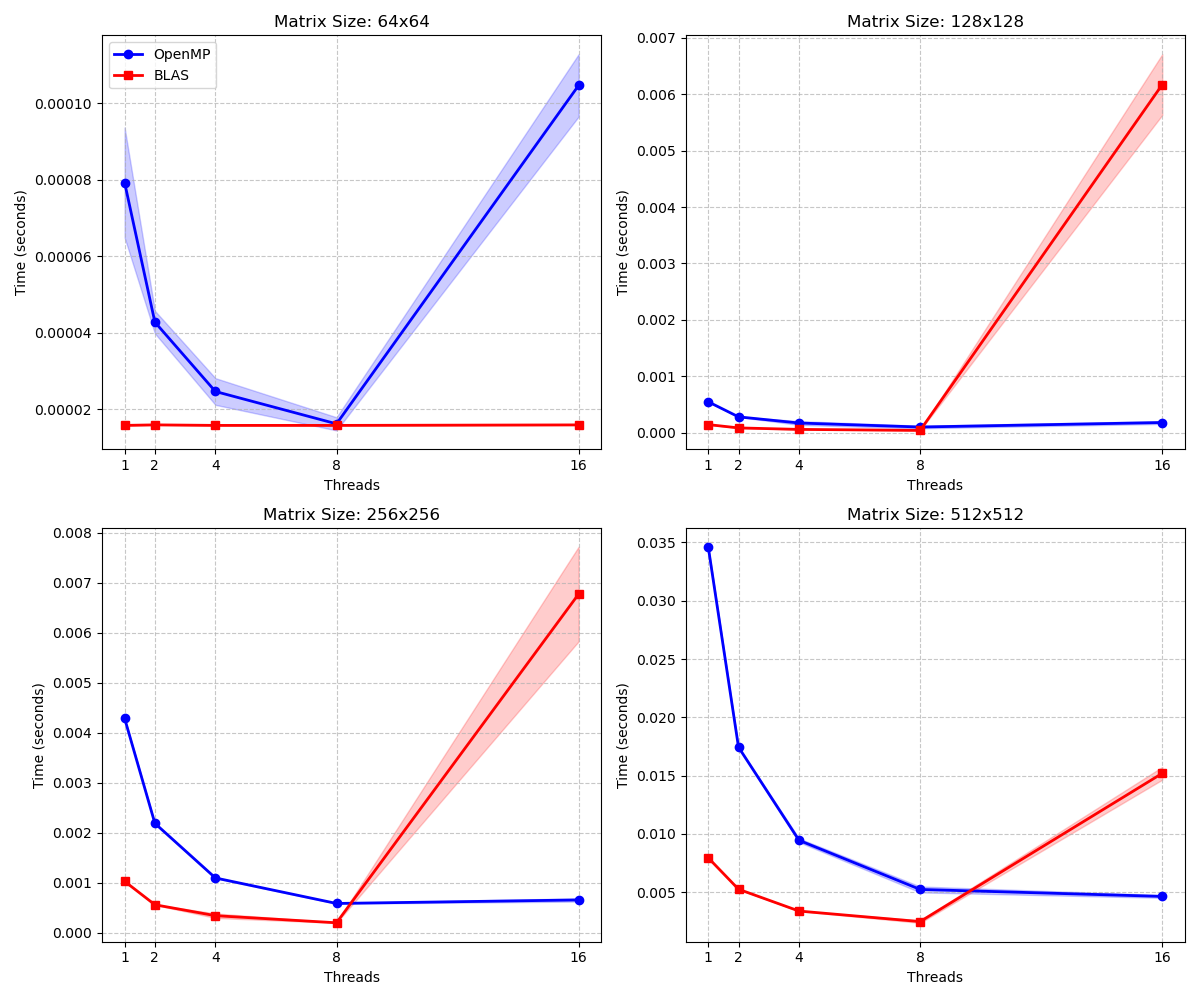
\includegraphics[width=0.90\textwidth]{../output/ExperienceGEMM/BLAS2/scaling_plot_advanced.png}
\caption{施加 CPU 亲和性约束后（BLAS2）的线程扩展性对比。
             在图中覆盖的 $64\times64$ 至 $512\times512$ 方阵上，并在 8 个物理线程配置下，\texttt{blas} 相对于同图中的其他实现给出最低测得时间。}
    \label{fig:blas2_scaling}
\end{figure}

\section{OpenMP blocked / packing 参数筛选补充}\label{app:blocked_pack_screening}

本附录补充正文第~\ref{sec:gemm_smt} 节之后 blocked 系列实验的完整 protocol。实验对象分为三条路径：\texttt{omp\_blocked}、\texttt{omp\_blocked\_packb} 与 \texttt{omp\_blocked\_packab}。筛选过程分为两轮：第一轮在 $64$、$128$、$256$ 与 $512$ 方阵上做小矩阵参数筛选，统一测试 1、2、4、8 个物理线程，默认每组重复 $1000$ 次；第二轮则对第一轮保留的少数候选在 $1024$ 与 $2048$ 上复测，用于确认大矩阵下的稳定性，并据此确定代表参数。

第一轮的候选空间并非完全自由搜索，而是按照正文中给出的 cache-resident 理论约束构造。\texttt{omp\_blocked} 测试 $\texttt{BlockSize}\in\{16,32,48,64,128,256\}$，其中前 3 个取值对应偏 L1 的候选，后 3 个取值对应偏 L2 的候选；\texttt{omp\_blocked\_packb} 只测试 $\texttt{BlockSize}\in\{16,32,48\}$，因为其目标是考察偏 L1 的 packed-$B$ 方案；\texttt{omp\_blocked\_packab} 则不再使用单一方块大小，而是从 $\texttt{PackM},\texttt{PackN}\in\{32,48,64,96,128\}$ 与 $\texttt{PackK}\in\{16,32,48,64,96\}$ 中保留满足 L1 footprint 约束的可行组合，再在这些组合上做第一轮筛选。

第一轮结束后，程序先对实验结果做聚合，再以参考规模（默认取最大筛选规模，即 $512$）下跨线程平均时间为依据，自动选出进入第二轮的少数候选。图~\ref{fig:blocked_small_screening} 仅展示 \texttt{omp\_blocked} 第一轮筛选在四组方阵上的按线程平均汇总；这一图的作用是观察 block size 的整体相对位置，而不是直接宣布统一最优参数。对应的候选汇总与第二轮复测结果均已保留，供后续复查。

\begin{figure}[H]
    \centering
    \includegraphics[width=0.88\textwidth]{../output/ExperienceGEMM/Blocked/omp_blocked/summary/screening_small_avg_over_threads.png}
    \caption{\texttt{omp\_blocked} 在 $64$ 至 $512$ 方阵上的小矩阵筛选汇总。
             图中对 1、2、4、8 个物理线程结果做平均后，可以看到 \texttt{BlockSize=64} 在较大方阵上更常落入较优区域，但不同矩阵尺寸与线程数下并不存在统一最优块大小。}
    \label{fig:blocked_small_screening}
\end{figure}

与图~\ref{fig:blocked_small_screening} 对应的 \texttt{omp\_blocked\_packb} 汇总 CSV 显示：
在当前保留的 $\texttt{BlockSize}\in\{16,32,48\}$ 范围内，$32$ 与 $48$ 基本稳定优于 $16$；
其中 $64\times64$ 上多由 $32$ 领先，$128\times128$ 上多由 $48$ 领先，
$256\times256$ 与 $512\times512$ 上则常在 $32$ 与 $48$ 之间切换。
对 \texttt{omp\_blocked\_packab} 而言，第一轮筛选后的第二轮候选集中在少数 L1-oriented 组合上，
最终保留的代表参数为 $(\texttt{PackM},\texttt{PackN},\texttt{PackK})=(32,128,16)$。

\section{AVX2单线程调优结果汇总}\label{app:avx2_tuning_results}

图~\ref{fig:avx2_kernelshape_line} 给出了一个代表性全连接工作负载 \texttt{fc\_forward\_mainstream\_nn / mlp\_fc1\_b32}（$32\times784\times128$）上的结果。对每种微内核形状，图中仅保留其对应的最佳 blocked 参数组合。

\begin{figure}[H]
    \centering
    \includegraphics[width=0.82\textwidth]{../output/ExperienceGEMM/GotoBLASBlocked/summary/plots/fc_forward_mainstream_nn_mlp_fc1_b32_gflops_by_kernel_shape.png}
    \caption{主流全连接工作负载 \texttt{mlp\_fc1\_b32} 上，不同 AVX2 微内核形状的单线程 GFLOPS 对比。横轴为 micro-kernel 形状，纵轴为该形状在最佳 blocked 参数下的中位 GFLOPS。}
    \label{fig:avx2_kernelshape_line}
\end{figure}

在该 workload 上，\texttt{4x16} 与 \texttt{8x8} 两种微内核形状明显领先：前者约为 $88.6$ GFLOPS，后者约为 $82.1$ GFLOPS，而其余形状大多仅落在 $43$ 至 $47$ GFLOPS 区间。

\begin{table}[H]
\centering
\begin{tabular}{p{0.24\textwidth}lrrrrrr}
\toprule
\textbf{工作负载族} & \textbf{最优内核} & $M_c$ & $N_c$ & $K_c$ &
\textbf{自定义} & \textbf{OpenBLAS} & \textbf{差距} \\
 & & & & & \textbf{($\mu$s)} & \textbf{($\mu$s)} & \\
\midrule
fc\_forward (b32) & 4x16 & 128 & 576 & 320 & 72.5  & 60.2 & $-17\%$ \\
fc\_forward (b64) & 4x16 & 192 & 512 & 256 & 132.6 & 110.1 & $-17\%$ \\
fc\_head (b32)    & 4x16 & --  & --  & --  & 4.76  & 1.14 & $-76\%$ \\
conv\_dx (b32)    & 8x8  & 160 & 640 & 288 & 744.3 & 647.3 & $-13\%$ \\
fc\_wide (b32)    & 4x16 & 128 & 768 & 256 & 136.5 & 122.2 & $-10\%$ \\
\bottomrule
\end{tabular}
\caption{AVX2单线程调优：各工作负载族的最佳配置及与OpenBLAS单线程的对比}
\label{tab:avx2_tuning_results}
\end{table}

从表~\ref{tab:avx2_tuning_results} 可见，在主流形状上，该实现与 OpenBLAS 的差距通常在 10 至 24\% 之间；而在很小的 $N$ 形状上（如 \texttt{fc\_head}），边界处理占比更高，差距会扩大到 66 至 78\%。

\section{AVX2 blocked-size 候选集合的推导}\label{app:blocked_size_tuning}

本附录补充正文中 $(M_r,N_r,K_c,M_c,N_c)$ 搜索空间缩减的依据。

\subsection{$m_r$ 与 $n_r$ 的实现相关推导}

当前微内核在每次 $p$ 迭代中执行
$
C_r(i,:) \leftarrow C_r(i,:) + A_r(i,p)\,B_r(p,:),
$
其中 $0 \le i < m_r$。这里 $B_r(p,:)$ 被一次性装入一个 AVX2 向量寄存器，$A_r(i,p)$ 则通过标量广播参与 FMA。语义上的 $m_r \times n_r$ 小块保持不变；SIMD lane 对应的是 $n_r$ 维度，寄存器方向因此与部分论文示例不同。

令 $N_{\text{vec}}$ 表示一个向量寄存器可容纳的标量数。对 AVX2 \texttt{float32}，有
$
N_{\text{vec}} = \frac{256}{32} = 8.
$
在参数优化语境中，$n_r$ 至少需要满足向量化粒度约束，并通常取为 $N_{\text{vec}}$ 的整数倍，即 $n_r = t\,N_{\text{vec}}$，其中 $t \in \mathbb{Z}_{\ge 1}$。若一个 $B_r(p,:)$ 在同一次迭代中由两个 YMM 寄存器共同承载，$n_r$ 也可以取 16。本文后续只考虑 $t \in \{1,2\}$，亦即 $n_r \in \{8,16\}$，暂不讨论 $n_r = 24,32$ 这类更宽的 $n$ 方向微内核。

$m_r$ 的约束来自吞吐隐藏和寄存器预算。BLIS 论文中关于微内核的基本条件可写为
$
m_r n_r \ge N_{\text{vec}} L_{\text{vfma}} N_{\text{vfma}} = 8 \times 4 \times 2 = 64,
$
其中 $L_{\text{vfma}}$ 是向量 FMA 的相关延迟，当前取 4 作为一阶建模值；$N_{\text{vfma}}$ 是每周期可发射的向量 FMA 数，当前取 2 作为一阶建模值，这给出了吞吐下界。

寄存器预算不能再写成与 $n_r$ 无关的统一形式，因为当 $n_r = 8$ 时，每一行累加器只占 1 个 YMM；当 $n_r = 16$ 时，每一行累加器占 2 个 YMM。令 $t = n_r / N_{\text{vec}} = n_r / 8$，则累加器寄存器数为 $m_r t$。因此，寄存器预算至少应写成依赖 $t$ 的形式：若一次迭代中只额外保留 1 个 $B$ 向量临时寄存器，则有
$
m_r t + 1 + \delta \le N_{\text{reg}} = 16;
$
若进一步针对 $n_r = 16$ 采用更保守的建模，即认为两个 $B$ 子向量都需要同时保留，则有
$
m_r t + t + \delta \le N_{\text{reg}} = 16.
$
其中 $N_{\text{reg}}$ 是可用向量寄存器数，$\delta$ 是留给广播、地址生成和调度的余量，且 $\delta \in [1,3]$。

因此必须分情况讨论。当 $n_r = 8$，即 $t = 1$ 时，吞吐下界给出 $m_r \cdot 8 \ge 64 \Rightarrow m_r \ge 8$，而乐观寄存器预算给出 $m_r + 1 + \delta \le 16$。当 $\delta \in [1,3]$ 时，可得到 $8 \le m_r \le 13$，因此当前建模下可保留
$
m_r \in \{8,9,10,11,12,13\}.
$
当 $n_r = 16$，即 $t = 2$ 时，吞吐下界给出 $m_r \cdot 16 \ge 64 \Rightarrow m_r \ge 4$。乐观寄存器预算变为 $2m_r + 1 + \delta \le 16$，更保守的预算写法则为 $2m_r + 2 + \delta \le 16$。按这组约束，$n_r = 16$ 时的可行 $m_r$ 区间更窄；若取稳妥候选，则可写成
$
m_r \in \{4,5,6\},
$
而 $m_r = 7$ 只在“$n_r = 16$ 且仅保留 1 个 $B$ 向量临时寄存器”的较乐观预算下才可能保留。

本节给出的可行域按 $n_r/8$ 分情况约束：

$$
\left\{
\begin{aligned}
&n_r \in \{8,16\},\\
&m_r n_r \ge 64,\\
&m_r \frac{n_r}{8} + 1 + \delta \le 16 \quad \text{(较乐观写法；当 } n_r=16 \text{ 时表示只保留 1 个 } B \text{ 向量临时寄存器)},\\
&m_r \frac{n_r}{8} + \frac{n_r}{8} + \delta \le 16 \quad \text{(较保守写法；对 } n_r=16 \text{ 等价于同时保留全部 } B \text{ 子向量)}.
\end{aligned}
\right.
$$

据此，原始可行域中的 $(m_r,n_r)$ 候选组合可写为
$$
\{(8,8),(9,8),(10,8),(11,8),(12,8),(13,8),(4,16),(5,16),(6,16)\},
$$
其中 $(7,16)$ 只在较乐观的寄存器预算下才可能保留，因此这里不将其放入默认候选集合。为控制后续搜索规模，本文后续固定保留的 $(m_r,n_r)$ 候选集合为
$
\{(8,8),(12,8),(13,8),(4,16),(5,16),(6,16)\}.
$

\subsection{$k_c$ 的缓存模型与候选生成}

\subsection*{B.2.1 基于 L1 的 $k_c$ 候选中心}

在给定 $(m_r,n_r)$ 后，$k_c$ 的角色是确定 packed $A_r \in \mathbb{R}^{m_r \times k_c}$ 与 $B_r \in \mathbb{R}^{k_c \times n_r}$ 的深度。本文先依据 L1 侧的面板占用关系构造候选中心，再结合对齐与 page-footprint 约束得到离散候选集合。

对 AVX2 \texttt{float32}，若以 cache line 为基本单位并记 L1 每路对应 1024B，则可把 $A_r$ 与 $B_r$ 面板的近似 set 压力分别写成与 $m_r k_c$、$n_r k_c$ 成正比的量。简化后，$A_r$ 方向的可用 set 预算上界可写为
$
C_{A_r}^{\max}=\left\lfloor \frac{7}{1+n_r/m_r} \right\rfloor,
$
再由此得到候选中心
$
k_c^{\text{center}} \approx \frac{1024\,C_{A_r}^{\max}}{m_r}.
$

$k_c^{\text{center}}$ 在本文中只作为当前硬件上的候选中心。当前微内核在每个 $p$ 迭代中先读取 $B_r(p,:)$，后广播 $A_r(:,p)$ 的标量；因此，L1 模型在本文中的作用是给出中心值与离散候选的生成起点。

\subsection*{B.2.2 基于 TLB / page-footprint 的 $k_c$ 约束}

仅由 L1 / set-mapping 关系确定 $k_c$ 仍然不够，因为随着 $k_c$ 增大，微面板与宏面板的 page footprint 都会同步扩大。若页大小为 $P$，则微面板级 footprint 近似满足

$$
\frac{m_r k_c S_{\text{data}}}{P} \lesssim E_{A_r,\mathrm{TLB}},
\qquad
\frac{k_c n_r S_{\text{data}}}{P} \lesssim E_{B_r,\mathrm{TLB}},
$$

这类弱裁剪在本文中只作为提醒，因此后续改用宏面板级裁剪。为把 TLB 层实例化为可执行规则，这里暂定使用 $m_c=128$、$n_c=512$ 作为 provisional panel volumes；它们只服务于当前轮次的 TLB-aware pruning。对 $P=4096$，有

$$
\operatorname{pages}(A_c) \approx \left\lceil \frac{m_c k_c S_{\text{data}}}{P} \right\rceil
= \left\lceil \frac{128 \cdot k_c \cdot 4}{4096} \right\rceil
= \left\lceil \frac{k_c}{8} \right\rceil,
$$

$$
\operatorname{pages}(B_c) \approx \left\lceil \frac{k_c n_c S_{\text{data}}}{P} \right\rceil
= \left\lceil \frac{k_c \cdot 512 \cdot 4}{4096} \right\rceil
= \left\lceil \frac{k_c}{2} \right\rceil.
$$

当前机器的 L1 DTLB 和 L2 DTLB 条目数分别为 72 和 3072。由于 $B_c$ 的页数对本节候选远小于 L2 DTLB 容量，真正有区分度的裁剪来自线程私有的 $A_c$。为给栈、$C$ 块、代码和其他数据保留余量，这里取保守的有效预算 $E_{A,\mathrm{eff}}=0.75 \times 72 = 54$，并采用如下 pruning 规则：若某个候选使 $\operatorname{pages}(A_c) > 54$，则将其从第一轮实验集合中剔除；若 $\operatorname{pages}(A_c) \le 54$ 且 $\operatorname{pages}(B_c) \ll 3072$，则该候选通过当前 TLB 层检查。该层只承担近似过滤作用，不承担新的中心值生成。

\subsection*{B.2.3 综合 L1 与 TLB 约束的 $k_c$ 候选生成}

候选生成分两步进行。第一步，由 L1 模型围绕候选中心生成原始离散集合。若记 $g_k$ 为 $k_c$ 的实现对齐粒度，则有

$$
\mathcal{K}_{\mathrm{L1}}(m_r,n_r) = \mathrm{Align}_{g_k}\bigl(\{ \alpha\, k_c^{\text{center}}(m_r,n_r) : \alpha \in \mathcal{A}_k \}\bigr),
$$

其中 $g_k$ 由 packed panel 的步长与外层块循环粒度决定，$\mathcal{A}_k$ 表示围绕 1 的有限比例邻域。为控制第一轮搜索规模，这里取保守实例化 $g_k=32$、$\mathcal{A}_k=\{0.75,1.00,1.25\}$。

第二步，由 TLB / page-footprint 条件对 $\mathcal{K}_{\mathrm{L1}}(m_r,n_r)$ 做一次近似裁剪，得到第一轮实验集合

$$
\mathcal{K}_{\mathrm{pruned}}(m_r,n_r) \subseteq \mathcal{K}_{\mathrm{L1}}(m_r,n_r).
$$

这里的 $k_c^{\text{center}}$、$\mathcal{K}_{\mathrm{L1}}$ 和 $\mathcal{K}_{\mathrm{pruned}}$ 都依赖于给定的 $(m_r,n_r)$。后续实验可以对每个 $(m_r,n_r)$ 分别搜索，也可以把各个候选集合并成一个并集候选池，但层次关系保持不变：L1 先生成，TLB 再裁剪。

对第 B.1 节最终保留的 6 组 $(m_r,n_r)$ 候选，按 $C_{A_r}^{\max}=\left\lfloor \frac{7}{1+n_r/m_r} \right\rfloor$ 与 $k_c^{\text{center}} \approx \frac{1024\,C_{A_r}^{\max}}{m_r}$ 计算，可得到表~\ref{tab:appendix_kc_candidates}。表中先给出 $\mathcal{K}_{\mathrm{L1}}(m_r,n_r)$，再给出经 TLB 层筛查后的 $\mathcal{K}_{\mathrm{pruned}}(m_r,n_r)$；其中使 provisional $A_c$ 页数超过 54 的偏大候选被实际剔除。

\begin{table}[H]
\centering
\begin{tabular}{lcccl}
\toprule
\textbf{$(m_r,n_r)$} & $C_{A_r}^{\max}$ & $k_c^{\text{center}}$ & \textbf{$\mathcal{K}_{\mathrm{L1}}$} & \textbf{$\mathcal{K}_{\mathrm{pruned}}$} \\
\midrule
$(8,8)$   & 3 & 384.0 & $\{288,384,480\}$ & $\{288,384\}$ \\
$(12,8)$  & 4 & 341.3 & $\{256,352,416\}$ & $\{256,352,416\}$ \\
$(13,8)$  & 4 & 315.1 & $\{224,320,384\}$ & $\{224,320,384\}$ \\
$(4,16)$  & 1 & 256.0 & $\{192,256,320\}$ & $\{192,256,320\}$ \\
$(5,16)$  & 1 & 204.8 & $\{160,192,256\}$ & $\{160,192,256\}$ \\
$(6,16)$  & 1 & 170.7 & $\{128,160,224\}$ & $\{128,160,224\}$ \\
\bottomrule
\end{tabular}
\caption{$k_c$ 候选的生成与 TLB 裁剪结果}
\label{tab:appendix_kc_candidates}
\end{table}

这些 $\mathcal{K}_{\mathrm{pruned}}(m_r,n_r)$ 构成第一轮 $k_c$ 搜索候选。它们来自“当前硬件上的中心值 + 32 对齐 + 有限比例邻域”，再经一层 page-footprint / TLB 过滤；例如 $1.25$ 比例产生的 $k_c=480$ 在 $(8,8)$ 这一行中因 provisional $A_c$ 页数达到 60、超过有效 L1 DTLB 预算 54 而被剔除。

本节约束可概括为

$$
\left\{
\begin{aligned}
&C_{A_r} + C_{B_r} \le W_{L1} - 1,\\
&C_{A_r} \le \left\lfloor \frac{W_{L1}-1}{1+n_r/m_r} \right\rfloor,\\
&k_c^{\text{center}} \approx \frac{1024\,C_{A_r}}{m_r},\\
&\mathcal{K}_{\mathrm{L1}}(m_r,n_r) = \mathrm{Align}_{g_k}\bigl(\{ \alpha\, k_c^{\text{center}}(m_r,n_r) : \alpha \in \mathcal{A}_k \}\bigr),\\
&\mathcal{K}_{\mathrm{pruned}}(m_r,n_r) \subseteq \mathcal{K}_{\mathrm{L1}}(m_r,n_r).
\end{aligned}
\right.
$$

\subsection{单线程基础 $m_c/n_c$ 候选生成}

\subsection*{B.3.1 基于 cache 的 $m_c/n_c$ 约束}

$m_c$ 与 $n_c$ 建立在已经筛出的 $(m_r,n_r,k_c)$ 候选之上：给定微内核形状和沿 $k$ 方向的面板深度后，$m_c$ 决定 $A_c \in \mathbb{R}^{m_c \times k_c}$ 的私有工作集高度，$n_c$ 决定 $B_c \in \mathbb{R}^{k_c \times n_c}$ 的共享工作集宽度。本节据此把 cache / TLB 约束推进成单线程或弱并行情形下的基础候选集合。

$A_c$ 在当前实现中按线程私有工作集处理，$B_c$ 对应多线程路径中的共享读取面板，因此本节先按单线程基础候选讨论其体积。两者的字节规模分别为

$$
|A_c| = m_c k_c S_{\text{data}},
\qquad
|B_c| = k_c n_c S_{\text{data}}.
$$

基于 cache 层次，可写出最直接的尺度约束

$$
m_c k_c S_{\text{data}} \lesssim \rho_A S_{\text{private}},
\qquad
k_c n_c S_{\text{data}} \lesssim \rho_B S_{\text{shared}}.
$$

其中 $\rho_A,\rho_B \in (0,1)$ 是用于保留冲突、代码和其他工作集余量的建模系数；这些关系式给出 $m_c^{\max}$ 与 $n_c^{\max}$ 的基础尺度上界。对当前机器，单线程基础建模中取每核私有 L2 容量 $S_{\text{private}}=1\text{ MiB}$；为限制单个 $B_c$ 面板的预算，再取保守的 effective shared-cache budget $\rho_B S_{\text{shared}} = 1\text{ MiB}$。再令 $\rho_A = 1/4$，则有

$$
m_c^{\max}(k_c) \approx \frac{\rho_A S_{\text{private}}}{k_c S_{\text{data}}}
= \frac{256\text{ KiB}}{4k_c}
= \frac{65536}{k_c},
$$

$$
n_c^{\max}(k_c) \approx \frac{\rho_B S_{\text{shared}}}{k_c S_{\text{data}}}
= \frac{1\text{ MiB}}{4k_c}
= \frac{262144}{k_c}.
$$

因此，cache 层在本节中的角色是给出随 $k_c$ 变化的基础尺度上界 $m_c^{\max}(k_c)$ 与 $n_c^{\max}(k_c)$，后续离散候选将在这些上界附近生成。

\subsection*{B.3.2 基于 TLB / page-footprint 的 $m_c/n_c$ 约束}

仅有 cache 尺度上界仍然不够，因为 $A_c$ 和 $B_c$ 的页覆盖会随 $m_c$ 与 $n_c$ 同步放大。若页大小为 $P$，则两者的近似页覆盖为

$$
\frac{m_c k_c S_{\text{data}}}{P},
\qquad
\frac{k_c n_c S_{\text{data}}}{P},
$$

对应的近似 TLB 裁剪条件可写为

$$
\frac{m_c k_c S_{\text{data}}}{P} \lesssim E_{A,\text{TLB}},
\qquad
\frac{k_c n_c S_{\text{data}}}{P} \lesssim E_{B,\text{TLB}}.
$$

这些式子在本节中承担第二层 pruning 的作用。当前代码没有控制 huge page、STLB、NUMA 归属或线程绑定，因此这里仍按近似约束处理。对当前机器，取 $P=4096$、L1 DTLB 条目数 72、L2 DTLB 条目数 3072，并采用保守的有效预算 $E_{A,\text{eff}}=54$ 与 $E_{B,\text{eff}}=192$；其中 $192$ 用于第一轮单线程基础候选生成时抑制过宽 $B_c$。则

$$
\operatorname{pages}(A_c) \approx \frac{m_c k_c}{1024},
\qquad
\operatorname{pages}(B_c) \approx \frac{k_c n_c}{1024}.
$$

于是，本节使用的 TLB-aware pruning 规则为：若某个 $m_c$ 候选使 $\operatorname{pages}(A_c) > 54$，则将其从 $\mathcal{M}_{\text{cache}}$ 中剔除；若某个 $n_c$ 候选使 $\operatorname{pages}(B_c) > 192$，则将其从 $\mathcal{N}_{\text{cache}}$ 中剔除。这里的 $E_{B,\text{eff}}$ 小于硬件 L2 DTLB 容量，用于在第一轮基础搜索中先裁掉过宽的 $B_c$ 面板。

\subsection*{B.3.3 综合 cache 与 TLB 约束的单线程基础候选生成}

对给定的 $(m_r,n_r,k_c)$ 候选，首先由 cache 上界生成原始离散集合

$$
\mathcal{M}_{\text{cache}}(m_r,n_r,k_c)
= \operatorname{Align}^{\downarrow}_{g_m}\bigl(\{\beta\, m_c^{\max}(k_c) : \beta \in \mathcal{A}_m\}\bigr),
$$

$$
\mathcal{N}_{\text{cache}}(m_r,n_r,k_c)
= \operatorname{Align}^{\downarrow}_{g_n}\bigl(\{\gamma\, n_c^{\max}(k_c) : \gamma \in \mathcal{A}_n\}\bigr),
$$

再由 TLB / page-footprint 做一次裁剪，得到

$$
\mathcal{M}_{\text{pruned}} \subseteq \mathcal{M}_{\text{cache}},
\qquad
\mathcal{N}_{\text{pruned}} \subseteq \mathcal{N}_{\text{cache}}.
$$

为控制第一轮单线程基础搜索规模，这里取 $g_m=32$、$g_n=64$，并令 $\mathcal{A}_m=\mathcal{A}_n=\{0.5,0.75,1.0\}$。这里的 $\operatorname{Align}^{\downarrow}$ 表示向下对齐到不超过目标值的最近粒度倍数。按同一规则，可对第 B.2 节保留下来的全部 $(m_r,n_r,k_c)$ 组合逐项构造单线程基础候选，如表~\ref{tab:appendix_round1_pruned} 所示。

\begin{table}[H]
\centering
\begin{tabular}{lclclcl}
\toprule
\textbf{$(m_r,n_r,k_c)$} & $m_c^{\max}$ & \textbf{$\mathcal{M}_{\text{cache}}$} & \textbf{$\mathcal{M}_{\text{pruned}}$} & $n_c^{\max}$ & \textbf{$\mathcal{N}_{\text{cache}}$} & \textbf{$\mathcal{N}_{\text{pruned}}$} \\
\midrule
$(8,8,288)$   & $227.6$ & $\{96,160,224\}$   & $\{96,160\}$   & $910.2$  & $\{448,640,896\}$     & $\{448,640\}$ \\
$(8,8,384)$   & $170.7$ & $\{64,128,160\}$   & $\{64,128\}$   & $682.7$  & $\{320,512,640\}$     & $\{320,512\}$ \\
$(12,8,256)$  & $256.0$ & $\{128,192,256\}$  & $\{128,192\}$  & $1024.0$ & $\{512,768,1024\}$    & $\{512,768\}$ \\
$(12,8,352)$  & $186.2$ & $\{64,128,160\}$   & $\{64,128\}$   & $744.7$  & $\{320,512,704\}$     & $\{320,512\}$ \\
$(12,8,416)$  & $157.5$ & $\{64,96,128\}$    & $\{64,96,128\}$ & $630.2$ & $\{256,448,576\}$     & $\{256,448\}$ \\
$(13,8,224)$  & $292.6$ & $\{128,192,288\}$  & $\{128,192\}$  & $1170.3$ & $\{576,832,1152\}$    & $\{576,832\}$ \\
$(13,8,320)$  & $204.8$ & $\{96,128,192\}$   & $\{96,128\}$   & $819.2$  & $\{384,576,768\}$     & $\{384,576\}$ \\
$(13,8,384)$  & $170.7$ & $\{64,128,160\}$   & $\{64,128\}$   & $682.7$  & $\{320,512,640\}$     & $\{320,512\}$ \\
$(4,16,192)$  & $341.3$ & $\{160,256,320\}$  & $\{160,256\}$  & $1365.3$ & $\{640,1024,1344\}$   & $\{640,1024\}$ \\
$(4,16,256)$  & $256.0$ & $\{128,192,256\}$  & $\{128,192\}$  & $1024.0$ & $\{512,768,1024\}$    & $\{512,768\}$ \\
$(4,16,320)$  & $204.8$ & $\{96,128,192\}$   & $\{96,128\}$   & $819.2$  & $\{384,576,768\}$     & $\{384,576\}$ \\
$(5,16,160)$  & $409.6$ & $\{192,288,384\}$  & $\{192,288\}$  & $1638.4$ & $\{768,1216,1600\}$   & $\{768,1216\}$ \\
$(5,16,192)$  & $341.3$ & $\{160,256,320\}$  & $\{160,256\}$  & $1365.3$ & $\{640,1024,1344\}$   & $\{640,1024\}$ \\
$(5,16,256)$  & $256.0$ & $\{128,192,256\}$  & $\{128,192\}$  & $1024.0$ & $\{512,768,1024\}$    & $\{512,768\}$ \\
$(6,16,128)$  & $512.0$ & $\{256,384,512\}$  & $\{256,384\}$  & $2048.0$ & $\{1024,1536,2048\}$  & $\{1024,1536\}$ \\
$(6,16,160)$  & $409.6$ & $\{192,288,384\}$  & $\{192,288\}$  & $1638.4$ & $\{768,1216,1600\}$   & $\{768,1216\}$ \\
$(6,16,224)$  & $292.6$ & $\{128,192,288\}$  & $\{128,192\}$  & $1170.3$ & $\{576,832,1152\}$    & $\{576,832\}$ \\
\bottomrule
\end{tabular}
\caption{第一轮单线程基础候选中的 $M_c/N_c$ 裁剪结果}
\label{tab:appendix_round1_pruned}
\end{table}

表~\ref{tab:appendix_round1_pruned} 给出的 $\mathcal{M}_{\text{pruned}}$ 与 $\mathcal{N}_{\text{pruned}}$ 构成了单线程或弱并行情形下的基础候选集合。它们对应“cache 先给基础尺度，TLB 再裁掉偏大的点”这一两层结构。后续实验再讨论这些基础候选如何进一步收缩。

第一轮单线程 coarse screening 覆盖了全部保留的 $(m_r,n_r,k_c)$ 组合；在此基础上，只对局部优胜的 5 组 \texttt{KernelShape/Kc} 继续做第二轮精筛。第二轮使用的更密 $M_c/N_c$ 网格如表~\ref{tab:appendix_round2_grids} 所示。

\begin{table}[H]
\centering
\begin{tabular}{lll l p{0.23\textwidth} p{0.23\textwidth} r}
\toprule
\textbf{内核} & \textbf{$m_r$} & \textbf{$n_r$} & \textbf{$k_c$} & \textbf{$M_c$ 候选} & \textbf{$N_c$ 候选} & \textbf{组合数} \\
\midrule
\texttt{8x8}  & 8 & 8  & 288 & $\{96,128,160,192\}$ & $\{448,512,576,640\}$ & 16 \\
\texttt{8x8}  & 8 & 8  & 384 & $\{64,96,128\}$ & $\{320,384,448,512\}$ & 12 \\
\texttt{4x16} & 4 & 16 & 192 & $\{160,192,224,256,288\}$ & $\{640,768,896,1024\}$ & 20 \\
\texttt{4x16} & 4 & 16 & 256 & $\{128,160,192\}$ & $\{512,576,640,704,768\}$ & 15 \\
\texttt{4x16} & 4 & 16 & 320 & $\{96,128,160\}$ & $\{384,448,512,576\}$ & 12 \\
\bottomrule
\end{tabular}
\caption{第二轮精筛使用的 $M_c/N_c$ 候选网格}
\label{tab:appendix_round2_grids}
\end{table}

因此，第二轮总候选数为 $16+12+20+15+12=75$。这些组合在第一轮已知优胜区域附近补足中间点，从而提高单线程 blocked-size 结论的稳定性。

\section{线程感知 $kCacheBlockM/N_c$ 调优热图补充}\label{app:mc_nc_heatmap}

\begin{figure}[H]
    \centering
    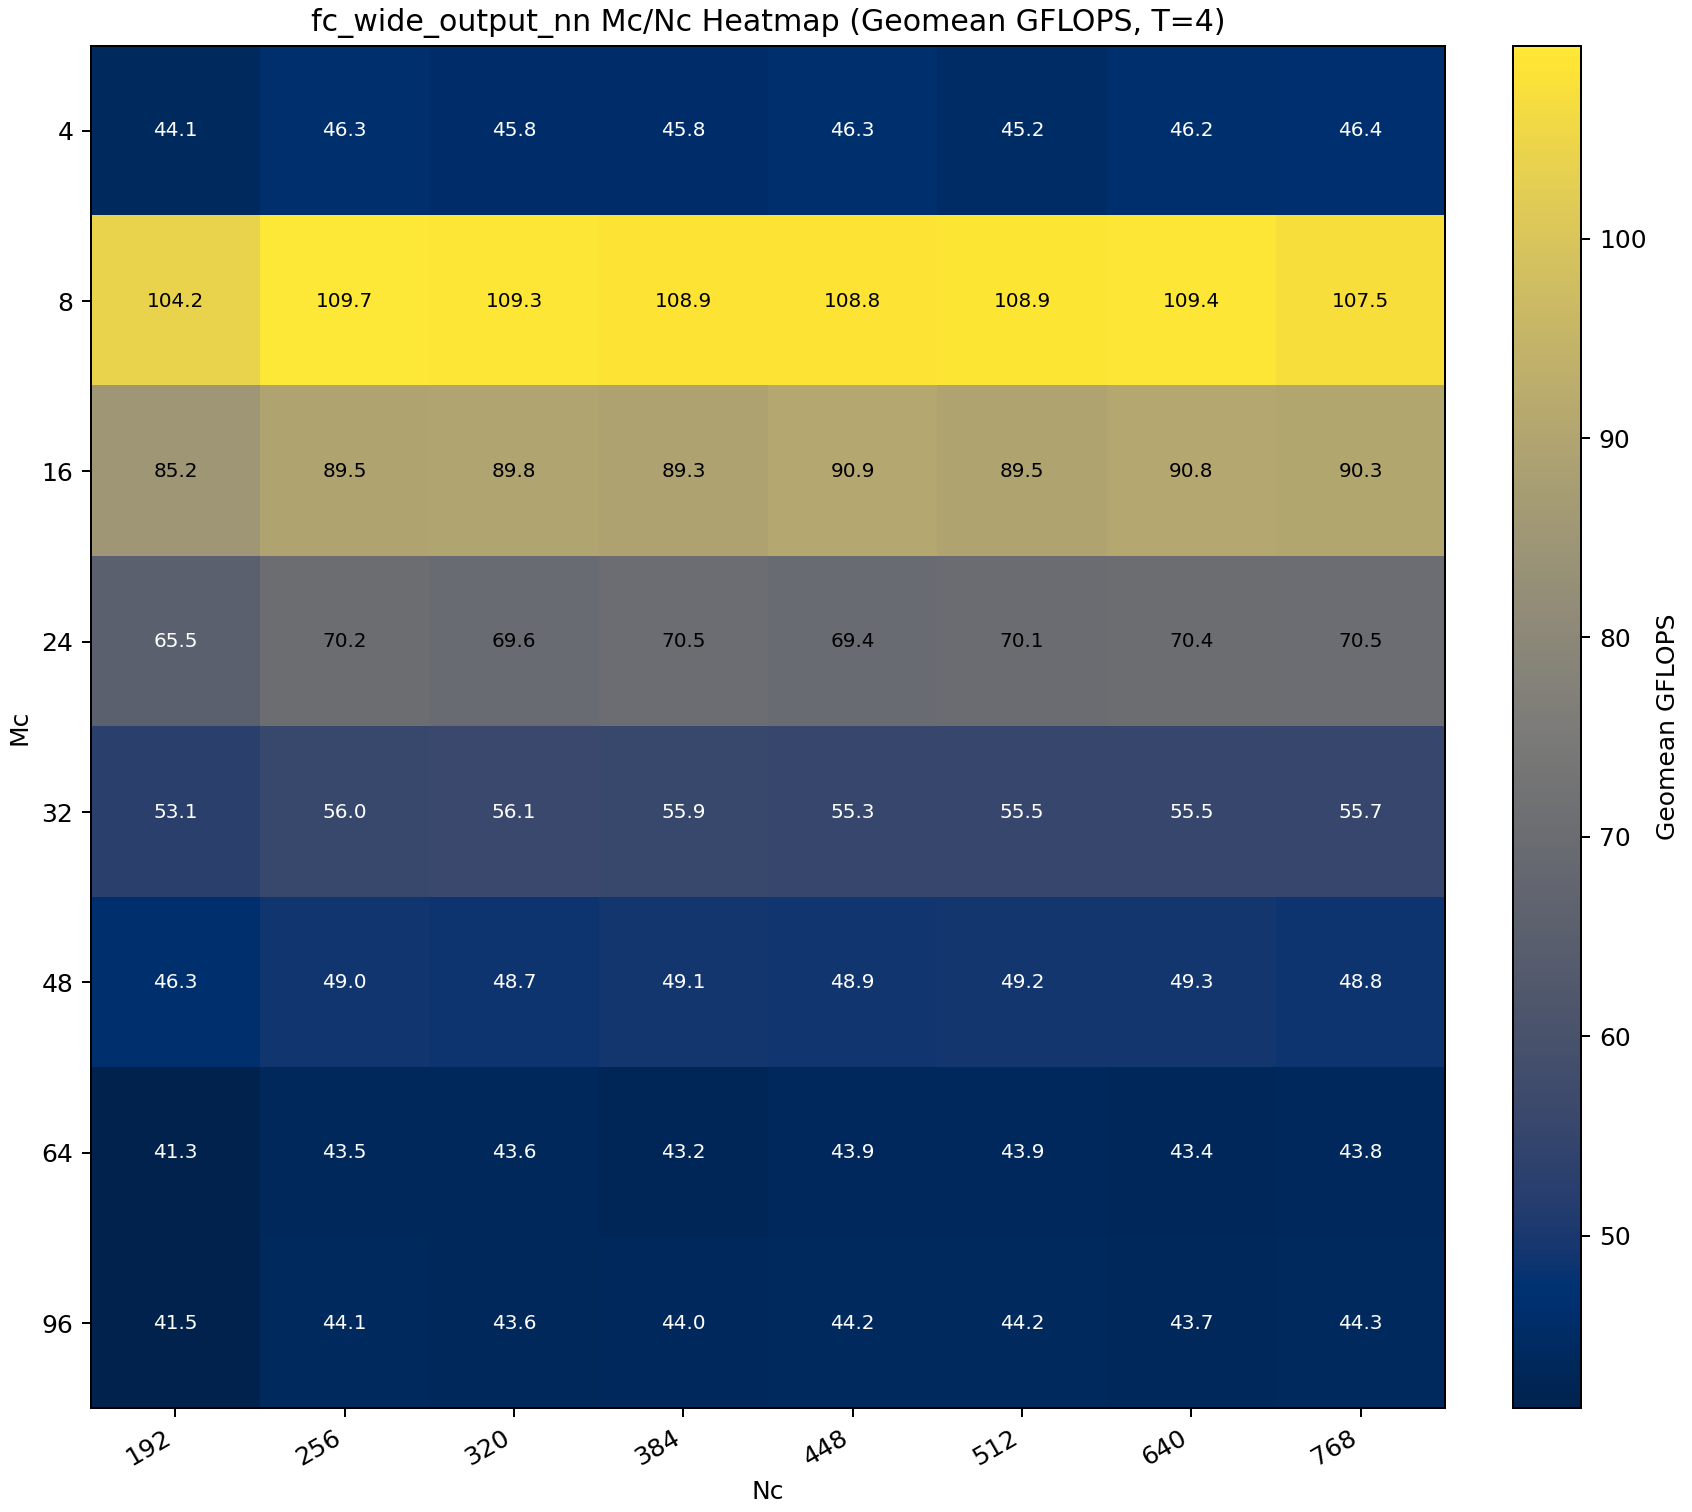
\includegraphics[width=0.84\textwidth]{../Docs/report/image-3.png}
    \caption{线程感知 \texttt{kCacheBlockM}/$N_c$ 调优的代表性热图（$T=4$，\texttt{fc\_wide\_output\_nn}）。
             高性能区域主要集中在 \texttt{kCacheBlockM}$=8$（有效 $M_c=64$）一行，而 $N_c$ 方向表现为相对平坦的平台。}
    \label{fig:mc_nc_heatmap_t4}
\end{figure}

\section{固定方阵上的线程扩展补充实验}\label{app:fixed_square_scaling}

除前述项目 workload 外，本文还对 64×64、128×128、256×256 和 512×512 四组固定方阵做了多实现线程扩展补充实验；图~\ref{fig:scaling_4way_all_impls} 汇总了 \texttt{blas}、\texttt{omp}、\texttt{omp\_blocked}、\texttt{omp\_blocked\_packab}、\texttt{omp\_gotoblas\_avx2} 以及 AVX-512 unroll+prefetch 路径在 1--8 个物理线程范围内的结果。

\begin{figure}[H]
    \centering
    \includegraphics[width=0.96\textwidth]{../output/ExperienceGEMM/scaling_plot_advanced_4way.png}
    \caption{固定方阵上的多实现线程扩展补充实验。四个子图分别对应 64×64、128×128、256×256 与 512×512，纵轴为执行时间，横轴为线程数。}
    \label{fig:scaling_4way_all_impls}
\end{figure}

图~\ref{fig:scaling_4way_all_impls} 显示，64×64 下 \texttt{blas} 基本保持近似单线程路径，线程数变化对其影响较小，而几条 OpenMP 路径通常要到 4--8 线程附近才接近这一水平；在 128×128 至 512×512 的区间里，\texttt{omp\_gotoblas\_avx2} 与 \texttt{omp\_gotoblas\_avx512\_unroll\_prefetch} 的时间曲线下降更快，其中后者在图中覆盖的固定方阵与 1--8 线程范围内整体上通常略优于 AVX2 路径。

\end{document}
